\documentclass[11pt,a4paper]{article}
\usepackage[margin=2.4cm]{geometry}
\usepackage[T1]{fontenc}
\usepackage{lmodern}
\usepackage{microtype}
\usepackage{amsmath,amssymb}
\usepackage{booktabs,multirow}
\usepackage{graphicx}
\usepackage{caption}
\usepackage{xcolor}
\usepackage[authoryear,round]{natbib}
\usepackage[colorlinks=true,linkcolor=blue!50!black,citecolor=blue!50!black,urlcolor=blue!50!black]{hyperref}
\graphicspath{{../figures/}}
\captionsetup{font=small,labelfont=bf}
\newcommand{\tabin}[1]{\resizebox{\linewidth}{!}{\input{tables/#1}}}

\title{Intraday Periodicity and Volatility Persistence, Revisited:\\
A Replication and Extension of Andersen \& Bollerslev (1997)\\ on Modern FX, Equity-Index and Crypto Data}
\author{Saksham Garg}
\date{October 2026}

\begin{document}
\maketitle

\begin{abstract}
\noindent
\citet{AB1997} showed that the deterministic intraday pattern in volatility distorts inference about volatility dynamics: GARCH models fitted to raw high-frequency returns give erratic, mutually inconsistent persistence estimates across sampling frequencies, and coherence is restored only after the periodic component is filtered out with a Flexible Fourier Form (FFF). We replicate the paper on 22 years of EUR/USD (the Deutschemark's successor), 15 years of an S\&P~500 index series and, as an original extension, eight years of BTC/USDT, all from free, key-less sources with a fully reproducible pipeline. The volatility patterns of the paper are still present and are strikingly stable across years. For EUR/USD the central result replicates almost exactly: raw-return persistence $\hat\alpha+\hat\beta$ exceeds one at 5--10 minutes and collapses at intermediate horizons (median minimum across 20 one-year windows 0.09), whereas FFF-filtered returns give persistence near 0.87--0.98 at every frequency; filtering improves aggregation consistency in 85\% of windows (Wilcoxon $p=0.0002$). The effect is weaker but significant for the S\&P~500 ($p=0.018$) and absent for BTC, whose intraday pattern is flat. We document that with tick-size discreteness A\&B's log-OLS estimator is biased by exact-zero returns and propose a Poisson pseudo-maximum-likelihood estimator of the same model. In strict walk-forward out-of-sample tests, periodicity-adjusted intraday GARCH beats raw intraday GARCH for all three assets (Diebold--Mariano $t=-10.7$, $-20.1$, $-4.0$) and modelling the pattern cuts time-of-day risk mis-allocation of a volatility-targeting trader from 33\% to 8\% (EUR/USD). In contrast, intraday \emph{mean}-return seasonality is economically irrelevant: in-sample ``significant'' intervals lose their edge out of sample, and the one statistically persistent effect (same-interval momentum) has a break-even cost an order of magnitude below the bid--ask spread.
\end{abstract}

\section{Introduction}
Return volatility in financial markets is not constant through the day. It follows a regular cycle tied to the opening and closing of trading venues, lunch breaks and scheduled news, and this cycle is highly correlated with trading volume and spreads \citep{Wood1985,Harris1986,AdmatiPfleiderer1988}. \citet{AB1997} --- henceforth A\&B --- made a deceptively simple point: because this cycle is so strong, any time-series model of intraday volatility that ignores it is misspecified, and the misspecification is severe enough to produce nonsense. In their one year of 5-minute Deutschemark--dollar (DM--\$) quotes and four years of S\&P~500 futures, GARCH(1,1) persistence estimates jumped from explosive ($\hat\alpha+\hat\beta>1$) at 5 minutes to half-lives of a few hours at 1--1.5 hours and back to weeks at 2 hours and longer. Temporal aggregation theory \citep{DrostNijman1993} says these numbers should describe the same process. Once the periodic component was estimated with a Flexible Fourier Form \citep{Gallant1981} and divided out, the estimates became coherent.

Almost thirty years later the paper's prescription --- \emph{deseasonalise before you model} --- is standard practice \citep{Engle2012,Boudt2011}, but its empirical premise has rarely been re-examined on modern markets with electronic trading, near-24-hour equity futures, algorithmic liquidity provision and crypto assets that never close. This study asks four questions:
\begin{enumerate}
\item \textbf{Replication.} Do A\&B's intraday volatility patterns and the frequency-dependent distortion of GARCH persistence still exist in modern data?
\item \textbf{Investigation.} How do returns, volatility and volume vary over the day, the week, volatility regimes and calendar time, and across asset classes?
\item \textbf{Out-of-sample relevance.} Does modelling the periodic component improve genuinely out-of-sample volatility forecasts and risk management?
\item \textbf{Mean returns.} Is there exploitable intraday seasonality in \emph{returns} once multiple testing and transaction costs are accounted for?
\end{enumerate}
We keep a strict separation between \emph{replication} (A\&B's specifications on modern analogues of their data, Section~\ref{sec:rep}), \emph{extensions} (new samples, assets, statistics and robustness, Sections~\ref{sec:results}--\ref{sec:rob}) and \emph{original research} (zero-robust estimation, out-of-sample tests and the BTC analysis, Sections~\ref{sec:method}, \ref{sec:oos} and \ref{sec:results}).

Our contributions are: (i) a fully reproducible, key-less pipeline including a data-driven correction of a previously undocumented timestamp convention in a widely used free data source; (ii) a replication showing that A\&B's FX result is remarkably durable while the equity result is attenuated; (iii) a Poisson pseudo-ML version of the FFF that remains valid when price discreteness produces exact-zero returns; (iv) walk-forward evidence that periodicity filtering is economically valuable for volatility forecasting and risk targeting; and (v) evidence that intraday \emph{mean} seasonality is not economically exploitable after costs.

\section{Literature}
\label{sec:lit}
\textbf{Intraday patterns.} The U-shape of equity volatility and volume is documented by \citet{Wood1985} and \citet{Harris1986} and rationalised by strategic trading models \citep{AdmatiPfleiderer1988}. FX volatility follows the rotation of trading centres around the globe \citep{Dacorogna1993}. \citet{AB1998} extend A\&B by modelling macroeconomic announcement effects, and \citet{Andersen2003} show that US releases at 08:30 New York time cause large, immediate FX price jumps.

\textbf{Intraday volatility modelling.} A\&B's FFF filter was followed by multiplicative component GARCH models for intraday equity data \citep{Engle2012}, by outlier-robust periodicity estimators \citep{Boudt2011}, and by heterogeneous-horizon models motivated exactly by the long-memory pattern A\&B uncovered in filtered returns \citep{Muller1997,Corsi2009}. \citet{TaylorXu1997} combine intraday seasonals with high-frequency volatility information for FX.

\textbf{Intraday return predictability.} \citet{Heston2010} find that a stock's return in a given half-hour predicts its return in the same half-hour on subsequent days; \citet{Gao2018} document intraday momentum in the market index. The multiple-testing problem in return-predictability research is emphasised by \citet{HarveyLiuZhu2016}.

\textbf{Econometric tools used here.} Quasi-ML GARCH inference \citep{Bollerslev1986,BollerslevWooldridge1992}; temporal aggregation \citep{DrostNijman1993}; Poisson pseudo-ML for multiplicative models with zeros \citep{SantosSilva2006}; robust forecast evaluation with noisy volatility proxies \citep{Patton2011}; Diebold--Mariano tests \citep{DieboldMariano1995}; HAC standard errors \citep{NeweyWest1987}; false-discovery-rate control \citep{BenjaminiHochberg1995}; block bootstrap \citep{Kunsch1989}.

\section{Hypotheses}
\label{sec:hyp}
All hypotheses, samples and splits were fixed before the corresponding results were computed.
\begin{description}
\item[H1 (replication).] Average absolute 5-minute returns display a pronounced, statistically significant intraday pattern: a multi-region pattern following the global trading-centre rotation for FX, and a U-shape with a post-cash-close drop for the equity index. Mean returns show no systematic pattern.
\item[H2 (replication).] MA(1)-GARCH(1,1) persistence estimated on raw intraday returns is inconsistent across sampling frequencies; after FFF filtering, the dispersion across frequencies of the implied half-life (in calendar minutes) falls.
\item[H3 (extension).] The intraday volume profile co-moves with the volatility profile.
\item[H4 (extension).] The shape of the periodic component depends on the volatility regime (A\&B's ``J-shape on high-volatility days'' for equities), on the day of the week and on scheduled announcements.
\item[H5 (extension).] Intraday mean-return seasonality is not economically exploitable out of sample after transaction costs.
\item[H6 (original).] Out of sample, volatility forecasts that model the periodic component beat forecasts that do not, and periodicity-filtered intraday GARCH beats raw intraday GARCH.
\item[H7 (original).] BTC, a 24/7 market, shows an FX-like geographic volatility pattern, and its activity shifted towards US equity hours around the January 2024 launch of US spot bitcoin ETFs.
\end{description}

\section{Data}
\label{sec:data}
\subsection{Sources and samples}
A\&B's data --- Olsen \& Associates' Reuters DM--\$ quotes for Oct~1992--Sep~1993 and CME S\&P~500 futures trades for 1986--1989 --- are not publicly available, so an exact numerical replication is impossible. We use the closest free, key-less analogues (Table~\ref{tab:data}):
\begin{itemize}
\item \textbf{EUR/USD}, 1-minute bid bars from HistData.com, 2004--2025. The euro replaced the Deutschemark in 1999, so EUR/USD is the direct successor of A\&B's DM--\$.
\item \textbf{S\&P~500}, the SPXUSD 1-minute series from HistData.com, 2010--2025, a contract-for-difference price that tracks the E-mini futures and trades almost 23 hours a day. It is a proxy for, not a copy of, A\&B's CME futures.
\item \textbf{BTC/USDT}, 5-minute spot klines with exchange volume from Binance's public archive, 2018--2025.
\item \textbf{Dukascopy} 1-minute bid candles (UTC-stamped) for independent validation only; the source rate-limits heavily, so it could not be used at scale.
\end{itemize}
Indices and currency pairs carry no survivorship bias in the usual sense; the BTC sample conditions on Bitcoin and Binance having survived, which we note as a limitation.

\begin{table}[t]
\centering\caption{Final samples after cleaning. ``Fresh'' is the share of 5-minute intervals containing at least one price update; ``Zero'' the share of returns exactly equal to zero.}
\label{tab:data}
\tabin{data_summary}
\end{table}

\subsection{Construction of returns}
Following A\&B, $R_{t,n}=100\,(\log p_{t,n}-\log p_{t,n-1})$ is the percentage return in 5-minute interval $n=1,\dots,N$ of day $t$. The price at grid time $g$ is the last observed price with timestamp $\le g$ (``previous tick''). A\&B interpolated linearly between the quotes either side of $g$, which uses a quote from \emph{after} $g$; we avoid this mild look-ahead.

\textbf{Trading days.} \emph{EUR/USD}: A\&B used 21:00--21:00 GMT days and dropped Friday 21:00 to Sunday 21:00 GMT. In our data every trading week opens at 17:00 Sunday and closes at 17:00 Friday New York time, i.e.\ 21:00 GMT in summer but 22:00 GMT in winter, so we define the FX day as 17:00--17:00 New York ($N=288$), the market's own rollover convention, and exclude the weekend analogously. If no fresh price exists at the session open, the first quote inside interval~1 is used as the base, keeping the weekend gap out of $R_{t,1}$. \emph{S\&P~500}: A\&B's window was 08:35--15:15 Chicago time, i.e.\ 09:35--16:15 New York: the cash session without the overnight-contaminated first five minutes, plus 15 minutes of post-close futures trading. Because SPXUSD trades around the clock we use the identical window ($N=80$). \emph{BTC}: 00:00--24:00 UTC, all seven days ($N=288$).

\textbf{Cleaning.} Days with fewer than 80\% fresh intervals or with a stale price (no update for 30 minutes) are dropped and logged, as are Christmas, New Year and NYSE early-close days for the non-crypto assets. Daily returns for the daily GARCH model run from the previous \emph{valid} close and include the overnight/weekend move.

\subsection{Validation, and a timestamp problem}
\label{sec:clock}
HistData documents its timestamps as ``EST without daylight saving''. A validation check showed this to be false: the 08:30 New York macro-release spike in EUR/USD and the 09:30 cash-open spike in SPXUSD sit at the \emph{same} raw clock time in summer and winter, so the clock follows New York daylight saving. Further, from 2019 onwards the clock runs one hour \emph{behind} New York in the weeks when the US is on daylight time but Europe is not, i.e.\ it follows European DST dates. Left uncorrected, every time-of-day result would be shifted by one hour in parts of the year. We therefore estimate the clock offset week by week from the observed weekly open, whose true New York time is known (17:00 for FX, 18:00 for the CME session), with the observed rule as a fallback.

The correction is verified independently. For every year and DST state, the 24-hour profile of mean absolute 1-minute returns is correlated with the pooled profile shifted by $-60$, $0$ and $+60$ minutes; a correct clock maximises the correlation at zero. This holds in 44 of 44 EUR/USD and 31 of 31 S\&P groups. Against Dukascopy's UTC-stamped data, 5-minute HistData returns on randomly drawn days have a correlation of 0.998 for both instruments and a standard-deviation ratio of 1.00.

\section{Methodology}
\label{sec:method}
\subsection{The A\&B model}
A\&B decompose the intraday return as
\begin{equation}
R_{t,n}=E(R_{t,n})+\frac{\sigma_t\,s_{t,n}\,Z_{t,n}}{N^{1/2}},\qquad Z_{t,n}\overset{iid}{\sim}(0,1),
\label{eq:model}
\end{equation}
where $\sigma_t$ is the daily volatility level, $s_{t,n}>0$ the periodic component and $Z$ an innovation independent of $\sigma$. The key assumptions are that $Z$ is independent of $\sigma$ and that $s$ is deterministic given $\sigma_t$. Equation~\eqref{eq:model} implies that the autocorrelation of $|R_{t,n}|$ combines a positive term driven by the persistence of $\sigma_t$ and a term driven by $\mathrm{Cov}(s_n,s_m)$, which is negative between intervals in the peak and the trough of the cycle (A\&B, eq.~4). That is why the raw correlogram oscillates with a daily period and why GARCH fitted to raw returns is misspecified.

\textbf{Daily volatility factor.} $\hat\sigma_t$ is the one-step-ahead conditional standard deviation from an MA(1)-GARCH(1,1) on daily returns; it uses returns up to day $t-1$ only.

\textbf{Flexible Fourier Form.} Squaring and taking logs of \eqref{eq:model} gives
$x_{t,n}\equiv 2\log|R_{t,n}-\bar R|-\log\hat\sigma_t^2+\log N=\log s_{t,n}^2+\log Z_{t,n}^2$, and A\&B regress $x$ by OLS on
\begin{equation}
f(\theta;\sigma_t,n)=\sum_{j=0}^{J}\sigma_t^j\Big[\mu_{0j}+\mu_{1j}\tfrac{n}{N_1}+\mu_{2j}\tfrac{n^2}{N_2}+\sum_{i}\lambda_{ij}I_{n=d_i}+\sum_{p=1}^{P}\big(\gamma_{pj}\cos\tfrac{2\pi pn}{N}+\delta_{pj}\sin\tfrac{2\pi pn}{N}\big)\Big],
\label{eq:fff}
\end{equation}
with $N_1=(N+1)/2$, $N_2=(N+1)(N+2)/6$, optional interval dummies $I_{n=d_i}$, and interactions with $\sigma_t^j$ that let the \emph{shape} of the pattern change with the volatility level. The estimate is normalised to have mean one: $\hat s_{t,n}=\exp(\hat f_{t,n}/2)/\overline{\exp(\hat f/2)}$ (A\&B eq.~A.4). For out-of-sample use the normalising constant comes from the fitting sample. As in A\&B we use $J=0,P=6$ for FX and $J=1,P=2$ with dummies for the last three intervals ($d=78,79,80$) for the S\&P~500.

\textbf{Filtered and standardised returns.} $\tilde R_{t,n}=R_{t,n}/\hat s_{t,n}$ (A\&B Table~4) and $\hat R_{t,n}=R_{t,n}/(\hat\sigma_t\hat s_{t,n})$ (Table~5).

\subsection{A zero-robust estimator}
The log transform fails for $R_{t,n}=\bar R$ and is badly behaved for returns of exactly zero, which are common when prices move in discrete ticks (Table~\ref{tab:data}: 6.9--7.0\% of EUR/USD and S\&P returns over the full sample). Dropping zeros, the only option for log-OLS, biases $\hat s$ upwards in quiet periods where zeros cluster. We instead estimate the same multiplicative model by \emph{Poisson pseudo-maximum likelihood} (PPML),
\begin{equation}
E\big[N(R_{t,n}-\bar R)^2/\hat\sigma_t^2\big]=\exp\{f(\theta;\hat\sigma_t,n)\},
\end{equation}
which is consistent whenever this conditional mean is correctly specified, whatever the distribution of $Z$, and treats zeros as ordinary observations \citep{SantosSilva2006}. It is estimated by Newton/IRLS with sandwich standard errors. In a Monte Carlo with A\&B's model and tick-rounded returns (13\%, 26\%, 40\% zeros), the maximum relative error of $\hat s$ is 2.1\%, 2.3\%, 2.9\% for PPML against 9.2\%, 13.3\%, 16.4\% for log-OLS (\texttt{tests/test\_methods.py}).

\subsection{GARCH at multiple frequencies}
Non-overlapping $k$-interval returns $R^{k}_{t,n}=\sum_{i=(n-1)k+1}^{nk}R_{t,i}$ for every divisor $k<N$ (17 frequencies for $N=288$, nine for $N=80$) are modelled as MA(1)-GARCH(1,1),
\[
R^k_{t,n}=\mu+\theta\epsilon_{t,n-1}+\epsilon_{t,n},\qquad
\sigma^2_{t,n}=\omega+\alpha\,\epsilon^2_{t,n-1}+\beta\,\sigma^2_{t,n-1},
\]
estimated by Gaussian QML with Bollerslev--Wooldridge robust standard errors. Both recursions are evaluated as linear filters, so the 1.6 million EUR/USD returns can be fitted in seconds. Persistence is summarised by $\alpha+\beta$, the half-life $-\log 2/\log(\alpha+\beta)$, and A\&B's mean and median lags, all converted to calendar minutes. Under temporal aggregation of weak GARCH \citep{DrostNijman1993}, $\alpha_{(k)}+\beta_{(k)}=(\alpha_{(1)}+\beta_{(1)})^k$, so the half-life in calendar time should not depend on $k$. We measure \emph{aggregation consistency} as the standard deviation across $k$ of $\log_{10}$ half-life (smaller is better).

\subsection{Inference}
Confidence bands for profiles use a 20-day moving-block bootstrap over days \citep{Kunsch1989}, which keeps the intraday shape and day-to-day volatility clustering intact. Mean-return $t$-statistics use Newey--West HAC errors, and the family of $N$ interval tests is controlled with the Benjamini--Hochberg false discovery rate at 5\%. Forecast comparisons use Diebold--Mariano tests on daily-averaged loss differentials with HAC errors.

\subsection{Out-of-sample design}
\label{sec:oosdesign}
Splits are chronological and fixed in advance: EUR/USD and S\&P~500 train $\le$2016, validate 2017--2019, test 2020--2025; BTC train $\le$2021, validate 2022, test 2023--2025. The FFF order $(P,J)$ is chosen once on the validation years from models fitted on training years. The test years are then forecast walk-forward: every January all parameters are re-estimated using only earlier years. Five variance forecasts $v_{t,n}$ are compared:
M0 flat ($\hat\sigma_t^2\cdot c$);
M1 historical profile ($\hat\sigma_t^2\cdot m_n$, $m_n$ the training mean of $R^2_{t,n}/\hat\sigma_t^2$);
M2 FFF ($\hat\sigma_t^2 e^{\hat f_{t,n}}/N$, PPML);
M3 FFF + intraday GARCH on filtered returns, $v=\hat s^2_{t,n}h_{t,n}$, A\&B's prescription; and
M4 GARCH on raw intraday returns.
M0--M2 use information available at the start of day $t$; M3--M4 also use returns up to interval $n-1$. The intraday GARCH models are estimated on the three years before each test year. Losses are QLIKE in its Gaussian quasi-likelihood form $R^2/v+\log v$, which is robust to the noise in $R^2$ as a proxy and defined when $R^2=0$ \citep{Patton2011}, and MSE.

\textbf{Look-ahead audit.} For every forecast of day $t$, interval $n$: $\hat\sigma_t$ uses parameters from earlier years and returns to $t-1$; profiles and FFF use earlier years; intraday $h$ uses parameters from earlier years and returns to $n-1$; trading signals use training statistics or returns from days before $t$.

\section{Replication}
\label{sec:rep}
The headline replication windows were fixed before any result was computed to mirror A\&B's sample lengths: one year of EUR/USD (Oct~2024--Sep~2025) and four years of S\&P~500 (2022--2025). All rolling windows are examined in Section~\ref{sec:rob}.

\textbf{Mean returns (A\&B Fig.~1).} Average 5-minute returns fluctuate around zero with violations of the confidence bands scattered across the day (Figure~\ref{fig:rep1} in the appendix), as in A\&B.

\textbf{Volatility profiles (A\&B Fig.~2, 6).} Figure~\ref{fig:profile} reproduces both of A\&B's patterns. EUR/USD volatility is lowest in the late Asian session, rises at the European open (02:00--03:00 New York), peaks in the London--New York overlap and decays after the London close. The sharpest feature, the 08:30 New York data-release interval, corresponds to the announcement effects A\&B mention but did not model. The S\&P~500 shows A\&B's Fig.~2b almost exactly: high at the open (about 0.093\%), a midday trough (about 0.052\%), a rise into the cash close and a collapse in the 15 minutes of post-close futures trading (intervals 78--80). The FFF tracks both closely; the 95\% block-bootstrap bands confirm that the pattern is overwhelmingly significant.

\begin{figure}[t]\centering
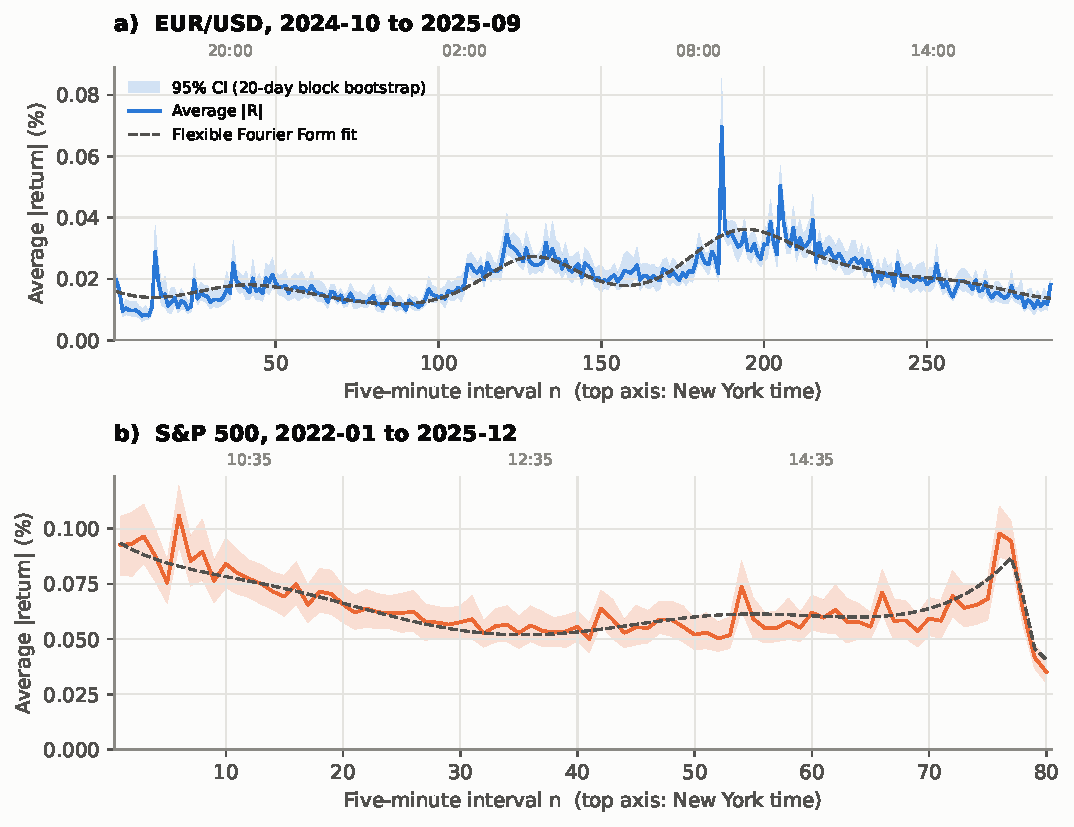
\includegraphics[width=0.92\linewidth]{rep_fig2_volatility_profile.pdf}
\caption{Average absolute 5-minute returns by interval with 95\% 20-day block-bootstrap bands and the FFF fit (PPML). Replicates A\&B Figs.~2 and~6.}
\label{fig:profile}
\end{figure}

\textbf{Correlograms (A\&B Figs.~3--5, 7).} Returns are close to white noise. Absolute returns show the oscillating correlogram predicted by A\&B's eq.~(4): for EUR/USD the autocorrelation rises to peaks at multiples of one day and turns \emph{negative} half a day apart, despite strong day-to-day volatility clustering (Figure~\ref{fig:corr}). After filtering, the oscillation disappears and a slow, hyperbolic decay emerges, the long-memory pattern that A\&B conjectured reflects several volatility components and that motivated HARCH and HAR models \citep{Muller1997,Corsi2009}. Standardised returns lose most of their remaining dependence. The S\&P~500 cycle is weaker.

\begin{figure}[t]\centering
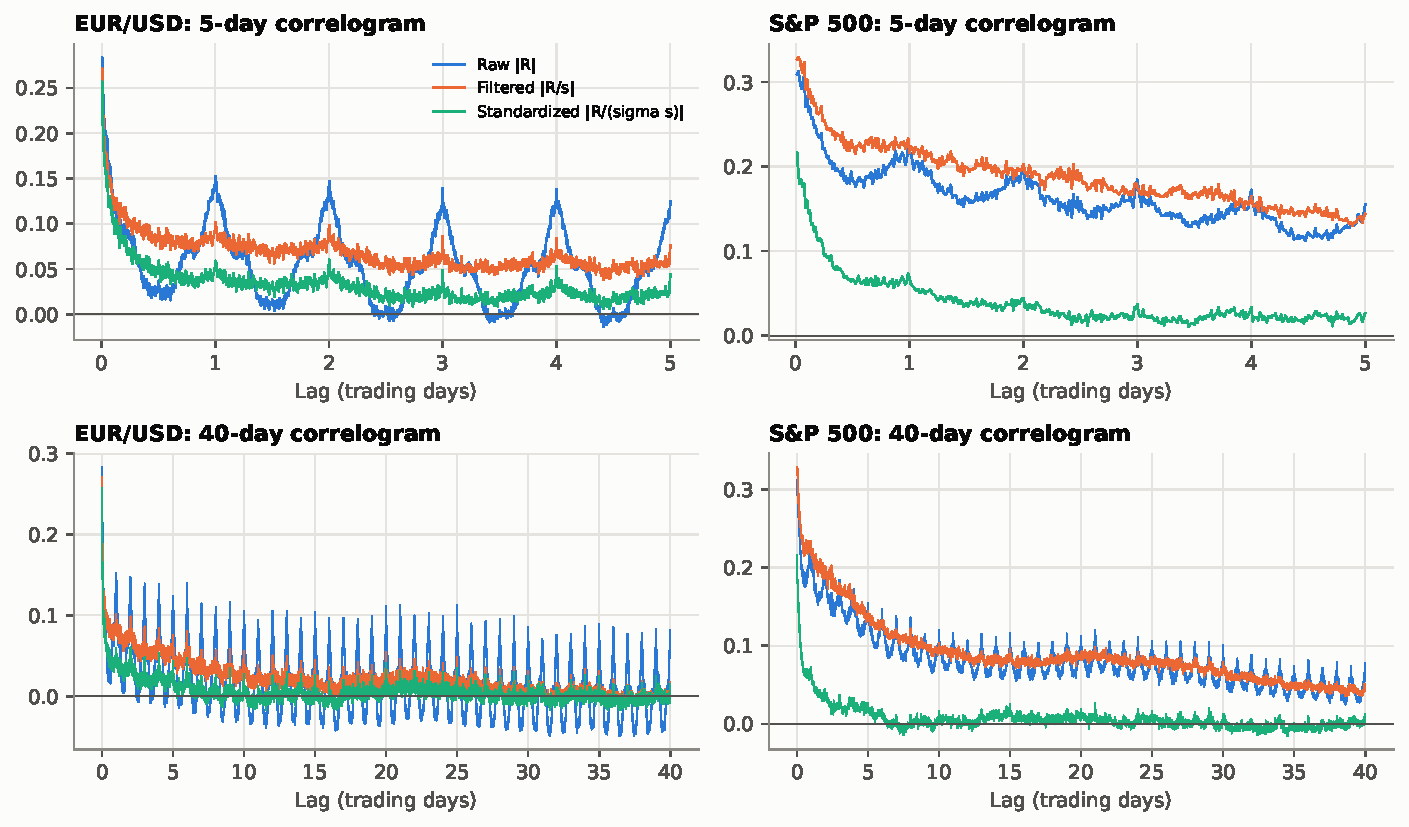
\includegraphics[width=0.95\linewidth]{rep_fig7_filtered_correlograms.pdf}
\caption{Correlograms of raw $|R|$, filtered $|R/\hat s|$ and standardised $|R/(\hat\sigma\hat s)|$. Replicates A\&B Fig.~7.}
\label{fig:corr}
\end{figure}

\textbf{Summary statistics (A\&B Table~1).} Table~\ref{tab:t1} compares selected columns. Magnitudes are close: the first-order autocorrelation of 5-minute absolute returns is 0.284 (A\&B 0.309) for EUR/USD and 0.309 (0.292) for the S\&P~500. A\&B's variance ratio for absolute returns $VR^A$ rises with $k$ as in the paper. Modern EUR/USD returns are less volatile and, at 5 minutes, more leptokurtic than the 1992--93 DM--\$ (kurtosis 50.8 vs.\ 21.5), consistent with announcement jumps in a market where quotes update instantly.

\begin{table}[t]\centering
\caption{A\&B Table~1, selected columns: this study (EUR/USD 2024--25; S\&P~500 2022--25) vs.\ A\&B (DM--\$ 1992--93; S\&P~500 futures 1986--89).}
\label{tab:t1}
\begin{minipage}{0.49\linewidth}\centering\small (a) EUR/USD vs.\ DM--\$\\[2pt]\resizebox{\linewidth}{!}{\begin{tabular}{rrrrrrrrr}
\toprule
 & \multicolumn{2}{c}{St.\ dev.\ (\%)} & \multicolumn{2}{c}{Kurtosis} & \multicolumn{2}{c}{$\rho_1^A$} & \multicolumn{2}{c}{$VR^A$} \\
\cmidrule(lr){2-3}\cmidrule(lr){4-5}\cmidrule(lr){6-7}\cmidrule(lr){8-9}
$k$ & here & A\&B & here & A\&B & here & A\&B & here & A\&B \\
\midrule
1 & 0.032 & 0.047 & 50.8 & 21.5 & 0.284 & 0.309 & 0.038 & 0.054 \\
2 & 0.044 & 0.066 & 27.3 & 16.6 & 0.299 & 0.313 & 0.065 & 0.071 \\
3 & 0.055 & 0.079 & 29.7 & 13.6 & 0.289 & 0.307 & 0.099 & 0.086 \\
4 & 0.063 & 0.089 & 21.3 & 14.0 & 0.303 & 0.287 & 0.120 & 0.099 \\
6 & 0.077 & 0.107 & 21.9 & 12.6 & 0.269 & 0.268 & 0.168 & 0.127 \\
8 & 0.089 & 0.121 & 19.1 & 9.1 & 0.266 & 0.272 & 0.205 & 0.149 \\
9 & 0.095 & 0.126 & 18.8 & 10.1 & 0.265 & 0.251 & 0.231 & 0.161 \\
12 & 0.107 & 0.148 & 16.4 & 11.0 & 0.192 & 0.229 & 0.311 & 0.193 \\
16 & 0.125 & 0.170 & 13.3 & 8.8 & 0.232 & 0.246 & 0.338 & 0.235 \\
18 & 0.133 & 0.178 & 14.1 & 10.6 & 0.189 & 0.193 & 0.369 & 0.260 \\
24 & 0.150 & 0.212 & 10.4 & 8.9 & 0.201 & 0.164 & 0.439 & 0.311 \\
32 & 0.174 & 0.246 & 9.9 & 9.2 & 0.165 & 0.171 & 0.586 & 0.373 \\
36 & 0.185 & 0.253 & 9.6 & 7.9 & 0.184 & 0.097 & 0.484 & 0.416 \\
48 & 0.211 & 0.300 & 6.8 & 5.9 & 0.099 & 0.075 & 0.706 & 0.487 \\
72 & 0.255 & 0.373 & 7.9 & 6.6 & 0.109 & 0.007 & 0.786 & 0.679 \\
96 & 0.304 & 0.423 & 6.5 & 5.2 & 0.082 & -0.025 & 0.895 & 0.653 \\
144 & 0.376 & 0.520 & 6.8 & 4.3 & 0.148 & -0.033 & 0.953 & 0.692 \\
\bottomrule
\end{tabular}}\end{minipage}\hfill
\begin{minipage}{0.49\linewidth}\centering\small (b) S\&P~500\\[2pt]\resizebox{\linewidth}{!}{\begin{tabular}{rrrrrrrrr}
\toprule
 & \multicolumn{2}{c}{St.\ dev.\ (\%)} & \multicolumn{2}{c}{Kurtosis} & \multicolumn{2}{c}{$\rho_1^A$} & \multicolumn{2}{c}{$VR^A$} \\
\cmidrule(lr){2-3}\cmidrule(lr){4-5}\cmidrule(lr){6-7}\cmidrule(lr){8-9}
$k$ & here & A\&B & here & A\&B & here & A\&B & here & A\&B \\
\midrule
1 & 0.100 & 0.104 & 60.0 & 29.3 & 0.309 & 0.292 & 0.052 & 0.099 \\
2 & 0.142 & 0.150 & 51.2 & 30.9 & 0.320 & 0.285 & 0.098 & 0.128 \\
4 & 0.200 & 0.212 & 60.1 & 33.2 & 0.308 & 0.232 & 0.186 & 0.179 \\
5 & 0.218 & 0.234 & 11.7 & 33.3 & 0.345 & 0.243 & 0.213 & 0.205 \\
8 & 0.282 & 0.299 & 41.7 & 22.2 & 0.295 & 0.207 & 0.337 & 0.261 \\
10 & 0.311 & 0.339 & 17.1 & 21.2 & 0.294 & 0.211 & 0.393 & 0.300 \\
16 & 0.399 & 0.437 & 22.3 & 26.6 & 0.224 & 0.135 & 0.546 & 0.405 \\
20 & 0.451 & 0.499 & 21.1 & 27.4 & 0.234 & 0.114 & 0.609 & 0.463 \\
40 & 0.650 & 0.728 & 18.3 & 16.2 & 0.248 & 0.148 & 0.810 & 0.673 \\
\bottomrule
\end{tabular}}\end{minipage}
\end{table}

\textbf{GARCH persistence across frequencies (A\&B Tables~2--5).} This is the paper's central result, and for FX it replicates almost exactly (Table~\ref{tab:persist}, Figure~\ref{fig:persist}). On raw EUR/USD returns, $\hat\alpha+\hat\beta$ is 1.019 at 5 minutes and 1.005 at 10 minutes (A\&B: 1.015 and 1.003), i.e.\ nonstationary. It falls to 0.80 at 80 minutes ($k=16$; A\&B's minimum is 0.52 at $k=18$), with implied half-lives of about four hours, before recovering at longer horizons. Raw $\hat\alpha$ is ``too large'' at high frequencies (0.19--0.39), exactly as A\&B observe. On filtered returns, persistence is 0.93--0.98 up to 4 hours and $\hat\alpha$ stabilises around 0.10. Standardised returns show the sharp decline in persistence with $k$ that A\&B report in Table~5. For the S\&P~500 in 2022--25, by contrast, raw persistence is already close to one at all frequencies and filtering changes little. Section~\ref{sec:rob} shows that this headline window is a weak case: over all years the S\&P effect is present but much smaller than the FX effect.

\begin{figure}[t]\centering
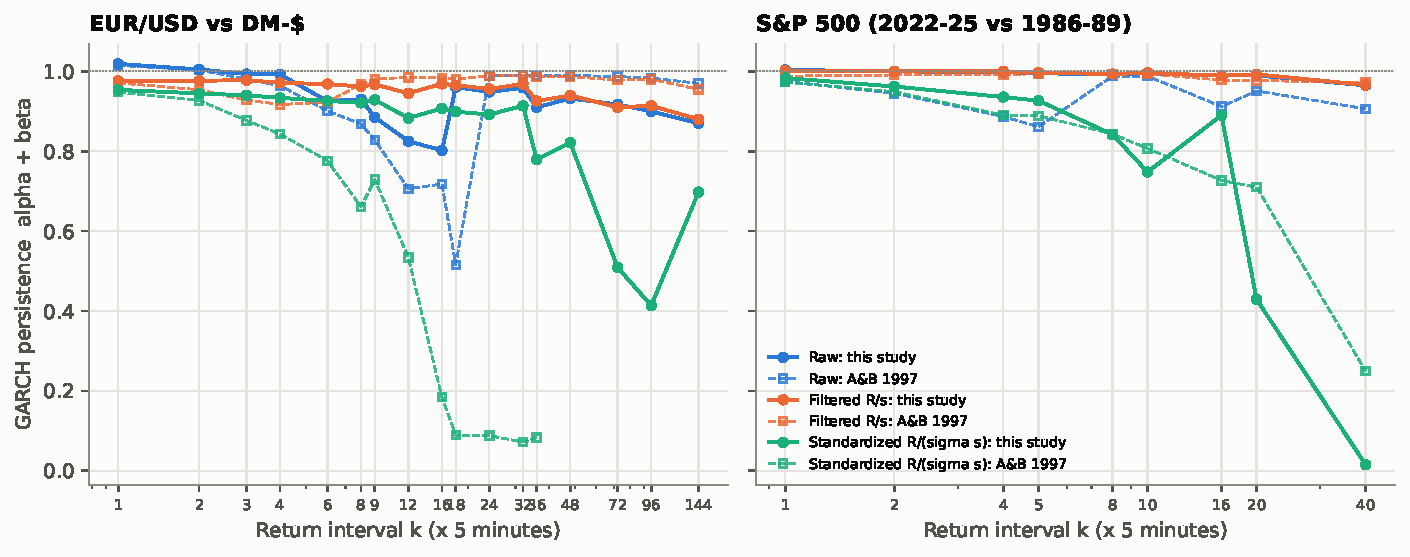
\includegraphics[width=\linewidth]{rep_fig_persistence_by_frequency.pdf}
\caption{GARCH persistence $\hat\alpha+\hat\beta$ by return interval for raw, filtered and standardised returns: this study (solid) vs.\ A\&B (dashed). Values above 1.05 are clipped.}
\label{fig:persist}
\end{figure}

\begin{table}[t]\centering
\caption{MA(1)-GARCH(1,1) by sampling frequency $k$ ($\times$5 min), EUR/USD Oct~2024--Sep~2025, with A\&B's DM--\$ values.}
\label{tab:persist}
\small\resizebox{0.85\linewidth}{!}{\begin{tabular}{rrrrrrrrr}
\toprule
 & \multicolumn{3}{c}{Raw $R$ (Table 2)} & \multicolumn{3}{c}{Filtered $R/\hat s$ (Table 4)} & \multicolumn{2}{c}{Standardised (Table 5)} \\
\cmidrule(lr){2-4}\cmidrule(lr){5-7}\cmidrule(lr){8-9}
$k$ & $\hat\alpha$ & $\hat\alpha+\hat\beta$ & A\&B & $\hat\alpha$ & $\hat\alpha+\hat\beta$ & A\&B & $\hat\alpha+\hat\beta$ & A\&B \\
\midrule
1 & 0.188 & 1.019 & 1.015 & 0.102 & 0.976 & 0.971 & 0.954 & 0.948 \\
2 & 0.215 & 1.005 & 1.003 & 0.089 & 0.976 & 0.954 & 0.945 & 0.927 \\
3 & 0.244 & 0.993 & 0.981 & 0.096 & 0.978 & 0.928 & 0.940 & 0.877 \\
4 & 0.315 & 0.992 & 0.964 & 0.101 & 0.971 & 0.917 & 0.934 & 0.843 \\
6 & 0.385 & 0.925 & 0.901 & 0.096 & 0.968 & 0.923 & 0.926 & 0.776 \\
8 & 0.307 & 0.930 & 0.868 & 0.101 & 0.962 & 0.968 & 0.921 & 0.661 \\
9 & 0.287 & 0.885 & 0.828 & 0.102 & 0.967 & 0.981 & 0.929 & 0.729 \\
12 & 0.189 & 0.825 & 0.706 & 0.089 & 0.945 & 0.985 & 0.883 & 0.534 \\
16 & 0.188 & 0.802 & 0.718 & 0.084 & 0.969 & 0.984 & 0.907 & 0.184 \\
18 & 0.047 & 0.960 & 0.516 & 0.090 & 0.965 & 0.981 & 0.899 & 0.089 \\
24 & 0.050 & 0.948 & 0.988 & 0.069 & 0.956 & 0.989 & 0.892 & 0.088 \\
32 & 0.056 & 0.959 & 0.991 & 0.083 & 0.968 & 0.990 & 0.914 & 0.072 \\
36 & 0.063 & 0.910 & 0.989 & 0.090 & 0.926 & 0.986 & 0.780 & 0.083 \\
48 & 0.044 & 0.932 & 0.990 & 0.067 & 0.940 & 0.987 & 0.821 & -- \\
72 & 0.049 & 0.917 & 0.987 & 0.064 & 0.910 & 0.978 & 0.509 & -- \\
96 & 0.044 & 0.900 & 0.983 & 0.064 & 0.914 & 0.980 & 0.414 & -- \\
144 & 0.079 & 0.870 & 0.970 & 0.079 & 0.880 & 0.955 & 0.698 & -- \\
\bottomrule
\end{tabular}}
\end{table}

\textbf{Estimator.} In these recent windows exact zeros are rare (2.4\% and 0.1\%) and PPML and log-OLS profiles nearly coincide (appendix Figure~\ref{fig:est}). PPML gives a better quasi-likelihood fit in every specification of Section~\ref{sec:rob}, and the gap matters most in the early, coarser-tick part of the sample.

\section{Results: investigation and extensions}
\label{sec:results}
\textbf{Cross-asset patterns.} On a common UTC clock (Figure~\ref{fig:cross}) EUR/USD carries the full trading-centre rotation; the S\&P~500 index session concentrates its volatility at the open and close; BTC is much flatter, with a broad maximum during US hours and no session boundaries. BTC's pattern is thus closer to FX's geographic rotation than to the equity U-shape, as H7 conjectured, but it is far weaker.

\begin{figure}[t]\centering
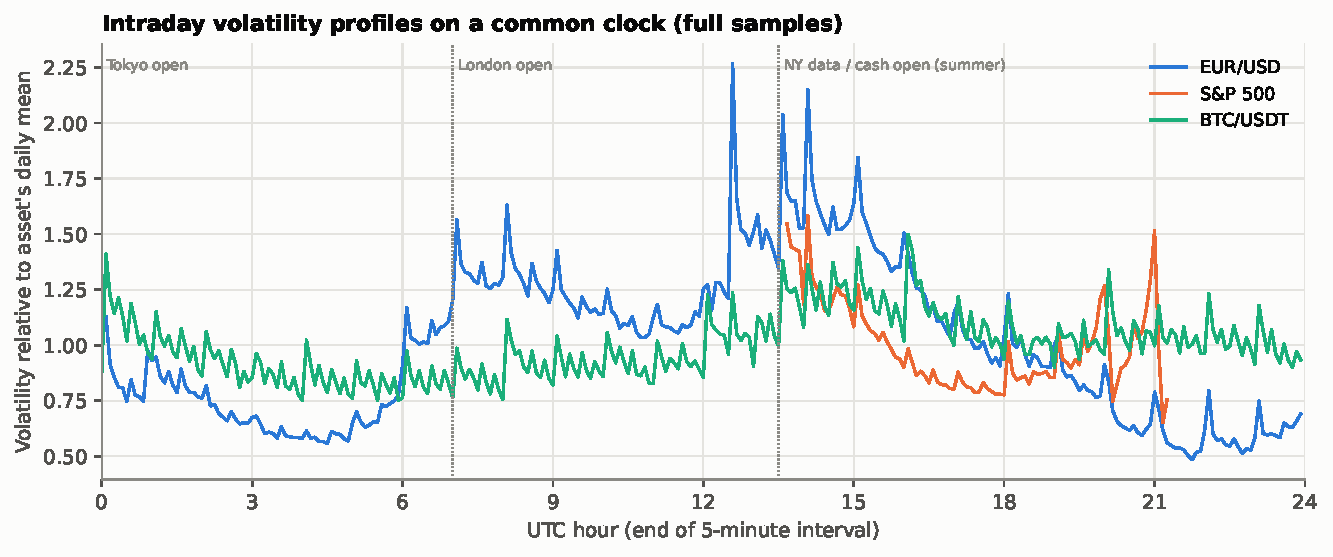
\includegraphics[width=0.95\linewidth]{ext_e1_cross_asset_profiles.pdf}
\caption{Normalised volatility profiles (1 = asset's daily mean) on a common UTC clock, full samples. EUR/USD and the S\&P~500 mix summer and winter, so New-York-anchored events appear at two UTC times.}
\label{fig:cross}
\end{figure}

\textbf{Volume (H3).} Only BTC has genuine free volume data. Its volume and volatility profiles correlate at 0.82 in logs, with an elasticity of volatility to volume of 0.59 across the 288 intervals; within days, the correlation between interval volume and $|R|$ averages 0.56 and is positive on every one of the 2,892 days (Figure~\ref{fig:vol}). H3 is supported for BTC; we cannot test it for FX and the index with free data.

\begin{figure}[t]\centering
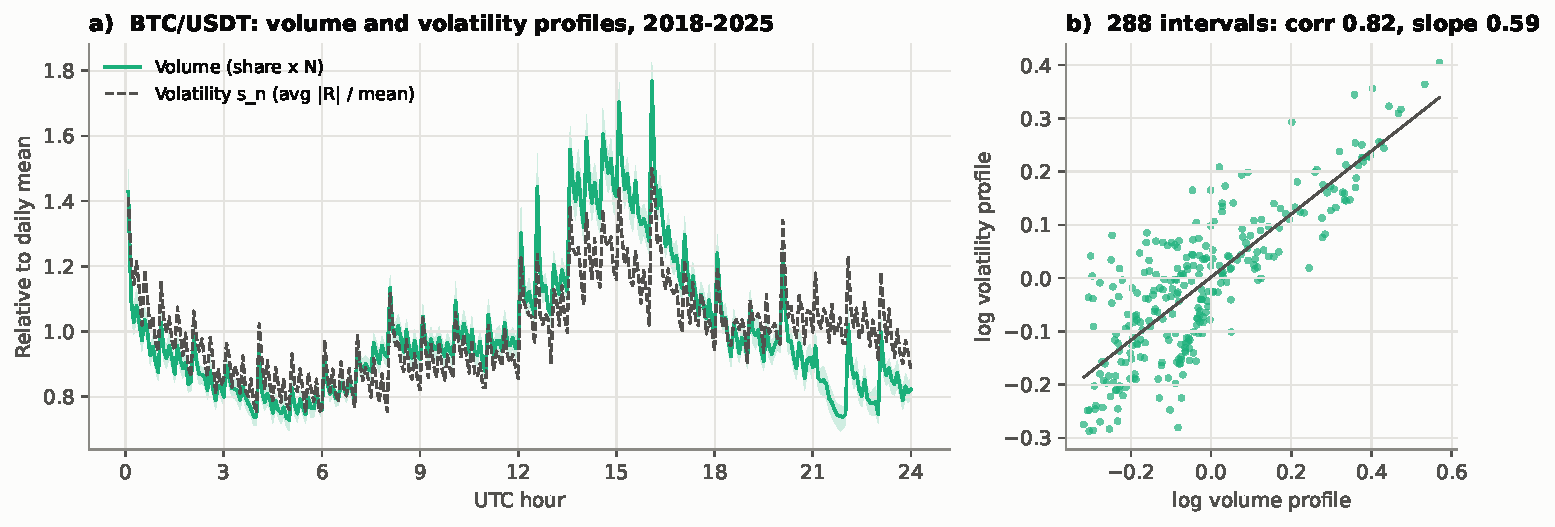
\includegraphics[width=\linewidth]{ext_e2_volume_volatility.pdf}
\caption{BTC/USDT: intraday volume and volatility profiles (95\% block-bootstrap band for volume) and their cross-interval relation.}
\label{fig:vol}
\end{figure}

\textbf{Day of week and announcements (H4).} Figure~\ref{fig:heat} shows time-of-day $\times$ day-of-week heatmaps. The FX 08:00--11:00 New York block is most volatile on Thursdays and Fridays; the BTC weekend is markedly quieter, without the US-hours peak. The 08:30 New York interval in EUR/USD has a volatility of 1.5 times the day's average on Mondays but \textbf{10.9 times} (95\% CI 9.6--12.3) on the first Friday of the month, when US payrolls are released (appendix Figure~\ref{fig:0830}), consistent with \citet{Andersen2003}.

\begin{figure}[t]\centering
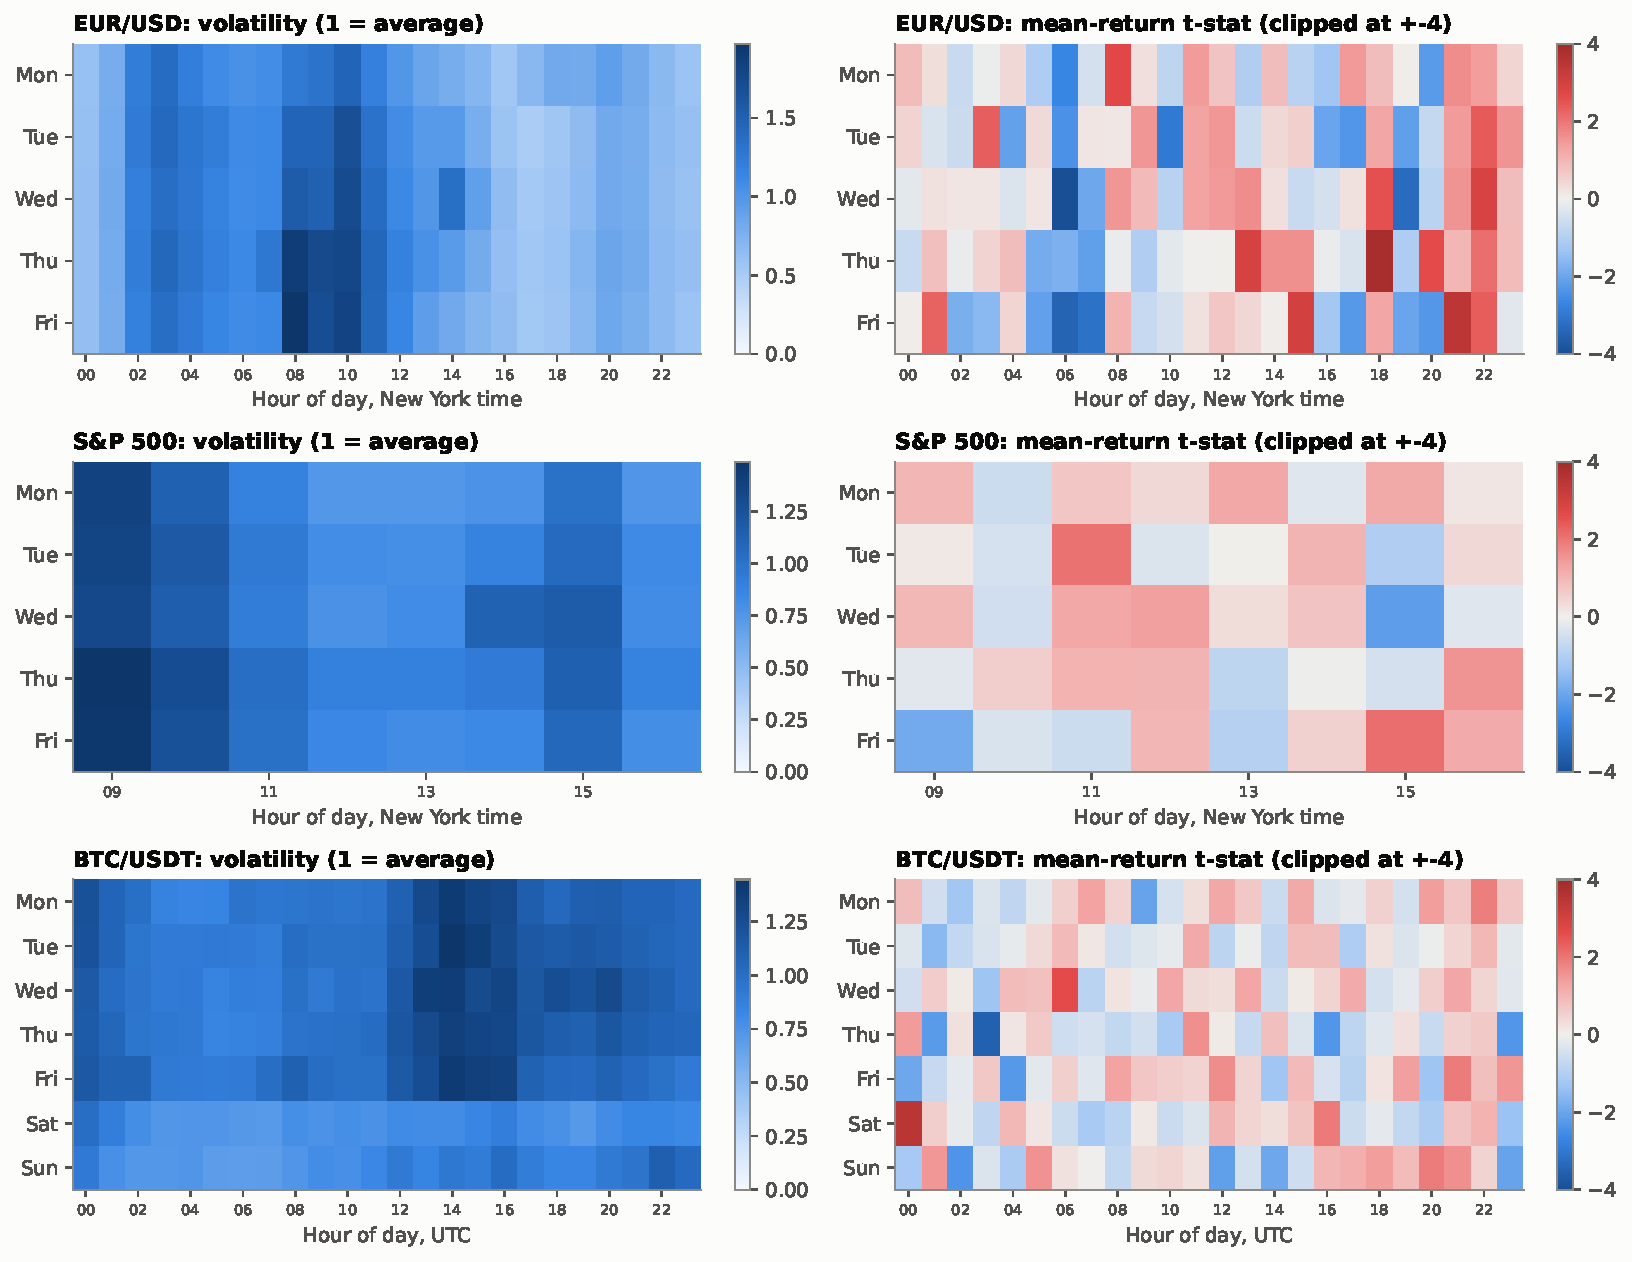
\includegraphics[width=\linewidth]{ext_e4_heatmaps_dow_hour.pdf}
\caption{Time-of-day $\times$ day-of-week heatmaps: volatility (left, 1 = average) and mean-return $t$-statistics (right, diverging scale, clipped at $\pm4$). For EUR/USD a row is the session \emph{ending} on that day (17:00--17:00 New York), so ``Mon'' includes Sunday evening.}
\label{fig:heat}
\end{figure}

\textbf{Volatility regimes (H4).} Splitting days into terciles of the \emph{ex ante} $\hat\sigma_t$ (parameters from training years only), the S\&P ratio of last-hour to first-hour volatility rises from 0.755 [0.727, 0.785] on low-volatility days to 0.810 [0.777, 0.846] on high-volatility days (Table~\ref{tab:jshape}): the right side of the U lifts relative to the left on volatile days, the direction A\&B describe as a J-shape tendency, although the open still dominates. For EUR/USD the corresponding ratio also rises (1.077 to 1.124), while for BTC it falls. The interaction terms in the S\&P FFF are individually borderline significant ($|t|\approx2$), as in A\&B.

\begin{table}[t]\centering
\caption{Last-hour / first-hour average $|R|$ by ex-ante volatility tercile, 95\% block-bootstrap CIs.}
\label{tab:jshape}
\small\begin{tabular}{llrrr}
\toprule
Asset & $\sigma_t$ tercile & Days & Last/first hour vol. & 95\% CI \\
\midrule
EUR/USD & Low & 1816 & 1.077 & [1.027, 1.133] \\
EUR/USD & Mid & 1815 & 1.078 & [1.037, 1.123] \\
EUR/USD & High & 1815 & 1.124 & [1.074, 1.176] \\
S\&P 500 & Low & 1217 & 0.755 & [0.727, 0.785] \\
S\&P 500 & Mid & 1216 & 0.767 & [0.743, 0.798] \\
S\&P 500 & High & 1216 & 0.810 & [0.777, 0.846] \\
BTC/USDT & Low & 964 & 0.913 & [0.867, 0.964] \\
BTC/USDT & Mid & 964 & 0.890 & [0.850, 0.934] \\
BTC/USDT & High & 964 & 0.864 & [0.826, 0.906] \\
\bottomrule
\end{tabular}
\end{table}

\textbf{Stability over calendar time.} The shape is remarkably stable. The correlation between each year's EUR/USD profile and the full-sample profile averages 0.96 (minimum 0.94) over 22 years, and 0.91 (minimum 0.82) for the S\&P~500. BTC's profile is less stable (0.82 on average, minimum 0.73), reflecting its changing investor base (appendix Figures~\ref{fig:stab}).

\textbf{Distributions.} Dividing returns by $\hat\sigma_t\hat s_n$ reduces the kurtosis of 5-minute S\&P returns from 53 to 10, but only from 40 to 33 for EUR/USD and from 133 to 113 for BTC (appendix Figure~\ref{fig:dist}). The remaining fat tails in FX are announcement jumps, which neither $\sigma_t$ nor a smooth $s_n$ can capture.

\textbf{Mean-return seasonality (H1, H5 in sample).} On training data, 48 of 288 EUR/USD intervals are significant at a naive 5\% level against 14.4 expected by chance; after Benjamini--Hochberg control, 19 remain. For the S\&P~500, 4 of 80 survive and for BTC none (Table~\ref{tab:meanret}). Their out-of-sample value is examined in Section~\ref{sec:oos}.

\begin{table}[t]\centering
\caption{Per-interval mean-return tests on training data (Newey--West $t$, BH false-discovery rate 5\%).}
\label{tab:meanret}
\small\begin{tabular}{lrrrrr}
\toprule
Asset & Training days & Intervals & Naive $p<0.05$ & Expected false & BH-FDR discoveries \\
\midrule
EUR/USD & 3250 & 288 & 48 & 14.4 & 19 \\
S\&P 500 & 1525 & 80 & 7 & 4.0 & 4 \\
BTC/USDT & 1432 & 288 & 21 & 14.4 & 0 \\
\bottomrule
\end{tabular}
\end{table}

\textbf{BTC and the spot ETF (H7).} The share of weekday BTC return variance falling in US cash hours (09:30--16:00 New York) rose from 40.8\% in the two years before 11 January 2024 to 45.2\% in the two years after (difference 4.3 points, 95\% block-bootstrap CI 1.4--6.4); the volume share rose 2.8 points [0.8, 4.1]. However, the annual series (Figure~\ref{fig:btc}) shows that most of the shift happened in 2022--2023 (29\% in 2021, 38\% in 2022, 44\% in 2023), \emph{before} the ETFs started trading. The data therefore document a migration of BTC price discovery towards US hours but do not support attributing it to the ETF launch; a before/after comparison around the launch alone would have been misleading.

\begin{figure}[t]\centering
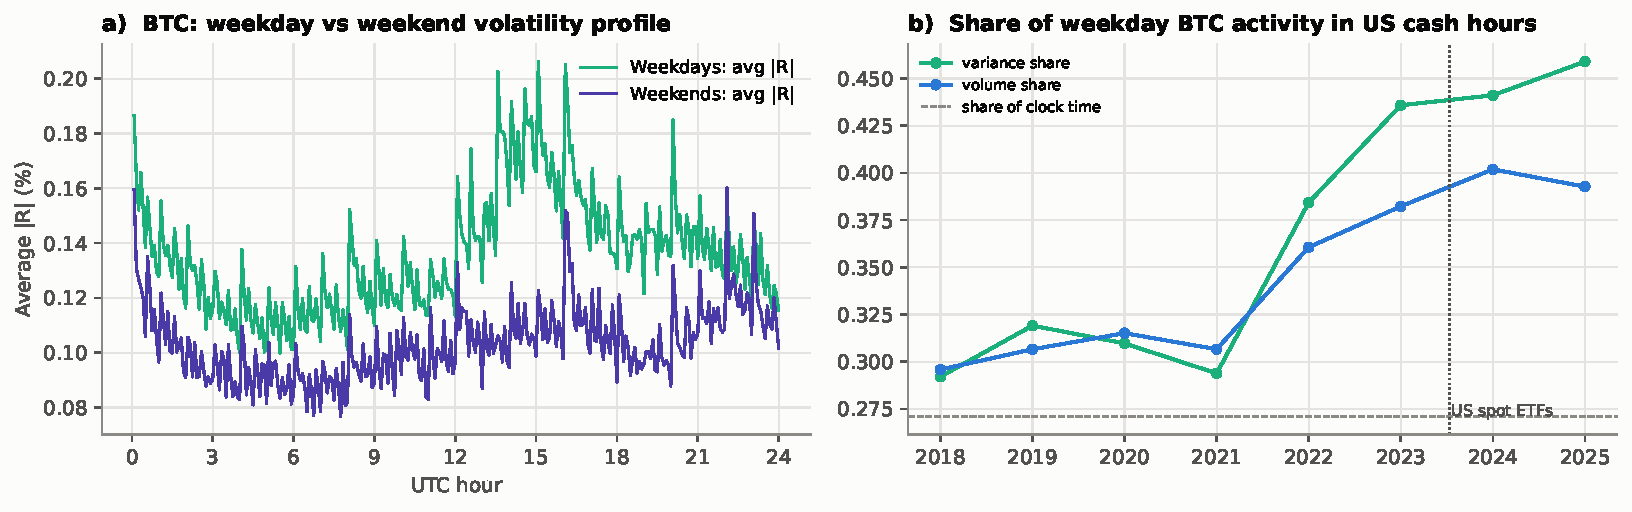
\includegraphics[width=\linewidth]{ext_e8_btc_weekend_etf.pdf}
\caption{BTC/USDT: (a) weekday vs.\ weekend profile; (b) share of weekday variance and volume in US cash hours by year, against the share of clock time (dashed).}
\label{fig:btc}
\end{figure}

\section{Robustness}
\label{sec:rob}
\textbf{All one-year windows (H2).} Table~\ref{tab:rob} and Figure~\ref{fig:robband} repeat the GARCH-by-frequency analysis in every one-year window: 20 EUR/USD windows (October--September; the window containing the 2023 data gap is skipped), 14 S\&P~500 and 8 BTC calendar years. For EUR/USD, filtering lowers the dispersion of log half-lives in 85\% of windows (one-sided Wilcoxon $p=0.0002$), and the median across windows of the minimum raw persistence is 0.09, against 0.87 after filtering. The median raw curve collapses from 1.0 at 5 minutes to 0.16 at 4 hours before jumping back, while the filtered curve stays near 0.95. For the S\&P~500 the effect is in the same direction and significant (86\% of windows, $p=0.018$) but small in magnitude: modern index volatility is dominated by day-to-day clustering, which keeps raw persistence high at all frequencies. For BTC filtering does not help ($p=0.23$), consistent with its weak periodic component.

\begin{table}[t]\centering
\caption{H2 across all one-year windows. Dispersion is the standard deviation across $k$ of $\log_{10}$ half-life (minutes).}
\label{tab:rob}
\tabin{rob_h2}
\end{table}

\begin{figure}[t]\centering
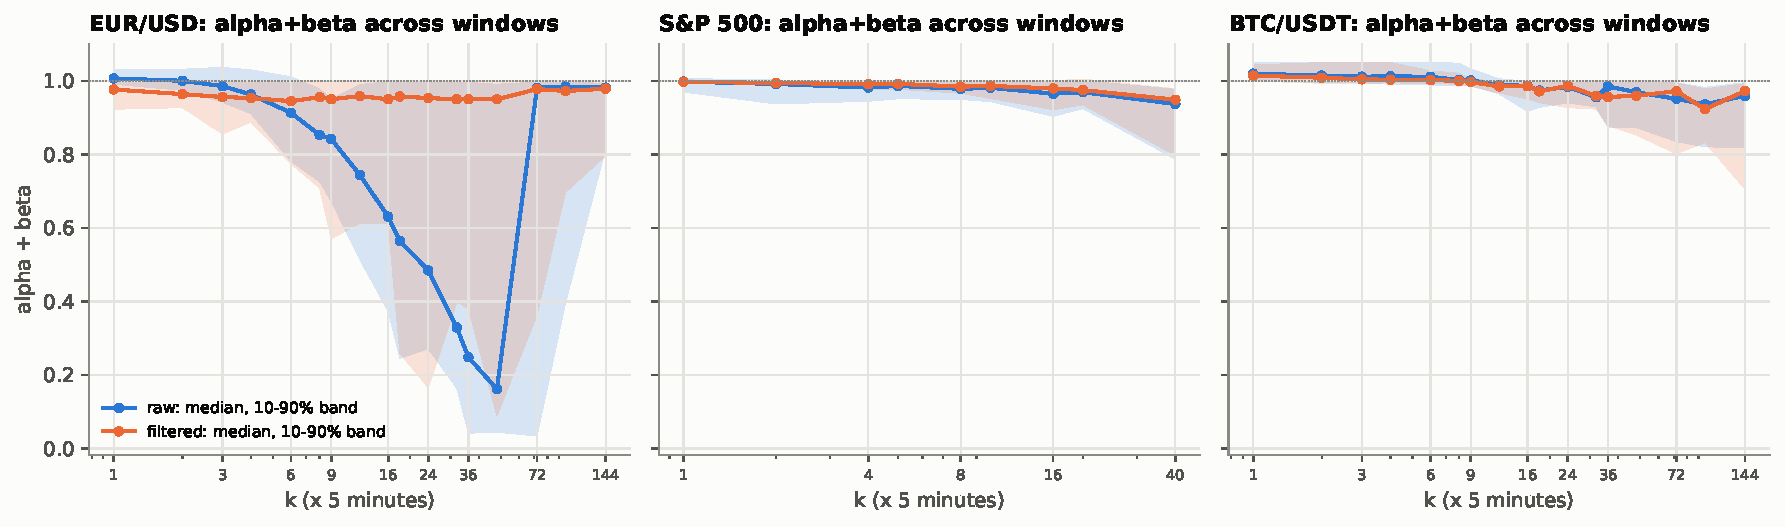
\includegraphics[width=\linewidth]{rob_r1_persistence_bands.pdf}
\caption{Median and 10--90\% band across one-year windows of $\hat\alpha+\hat\beta$ by frequency, raw vs.\ filtered returns.}
\label{fig:robband}
\end{figure}

\textbf{FFF specification.} Varying $P\in\{1,2,4,6,8\}$, $J\in\{0,1\}$ and the estimator on the headline windows (appendix Figure~\ref{fig:spec}), the filtered EUR/USD minimum persistence stays between 0.86 and 0.89 in every specification, so the replication result does not hinge on A\&B's choice $P=6$. PPML attains a better quasi-likelihood than log-OLS in all 20 comparisons. For the S\&P~500 the aggregation-consistency measure is sensitive to the specification, reinforcing that the equity result is fragile.

\textbf{Other checks.} The clock correction (Section~\ref{sec:clock}) and the source cross-check make data-timing artefacts an unlikely explanation for any time-of-day result. Results are reported for three assets, two decades and 17 frequencies rather than for a selected window.

\section{Out-of-sample analysis}
\label{sec:oos}
\textbf{Volatility forecasts (H6).} Table~\ref{tab:oos} and Figure~\ref{fig:oos} report walk-forward test-period losses. Modelling the intraday pattern is essential: every periodicity-aware model beats the flat forecast M0 with Diebold--Mariano $|t|>13$. Two further results stand out.
\begin{enumerate}
\item \textbf{A\&B's prescription works out of sample.} Periodicity-filtered intraday GARCH (M3) is the best model for all three assets and beats raw intraday GARCH (M4) with DM $t$-statistics of $-10.7$ (EUR/USD), $-20.1$ (S\&P~500) and $-4.0$ (BTC). Ignoring the periodic component in a dynamic intraday model is costly even when the model can react to the previous interval's return.
\item \textbf{A smooth FFF is not the best static profile when data are plentiful.} With 13 years of training data, the non-parametric historical profile (M1) beats the FFF (M2) for EUR/USD (DM $t=+5.6$) and the S\&P~500 ($+3.9$): averages over 3,000+ days have negligible estimation error and preserve sharp features such as the 08:30 spike, which a low-order Fourier series smooths away. The validation step chose $P=8$, the largest order considered, for both. For BTC, whose pattern is weaker and has shifted over time, the parsimonious FFF wins ($t=-14.1$).
\end{enumerate}
Under MSE the differences are smaller and mostly insignificant, as expected for a loss dominated by a few extreme squared returns \citep{Patton2011}.

\begin{table}[t]\centering
\caption{Out-of-sample 5-minute variance forecasts (test period, walk-forward). QLIKE is $R^2/v+\log v$ (lower is better). DM $t$: Diebold--Mariano statistic on daily loss differentials with HAC errors (negative = row model better). Risk error: mean absolute log deviation, across intervals, of realised from targeted risk.}
\label{tab:oos}
\tabin{oos_forecasts}
\end{table}

\begin{figure}[t]\centering
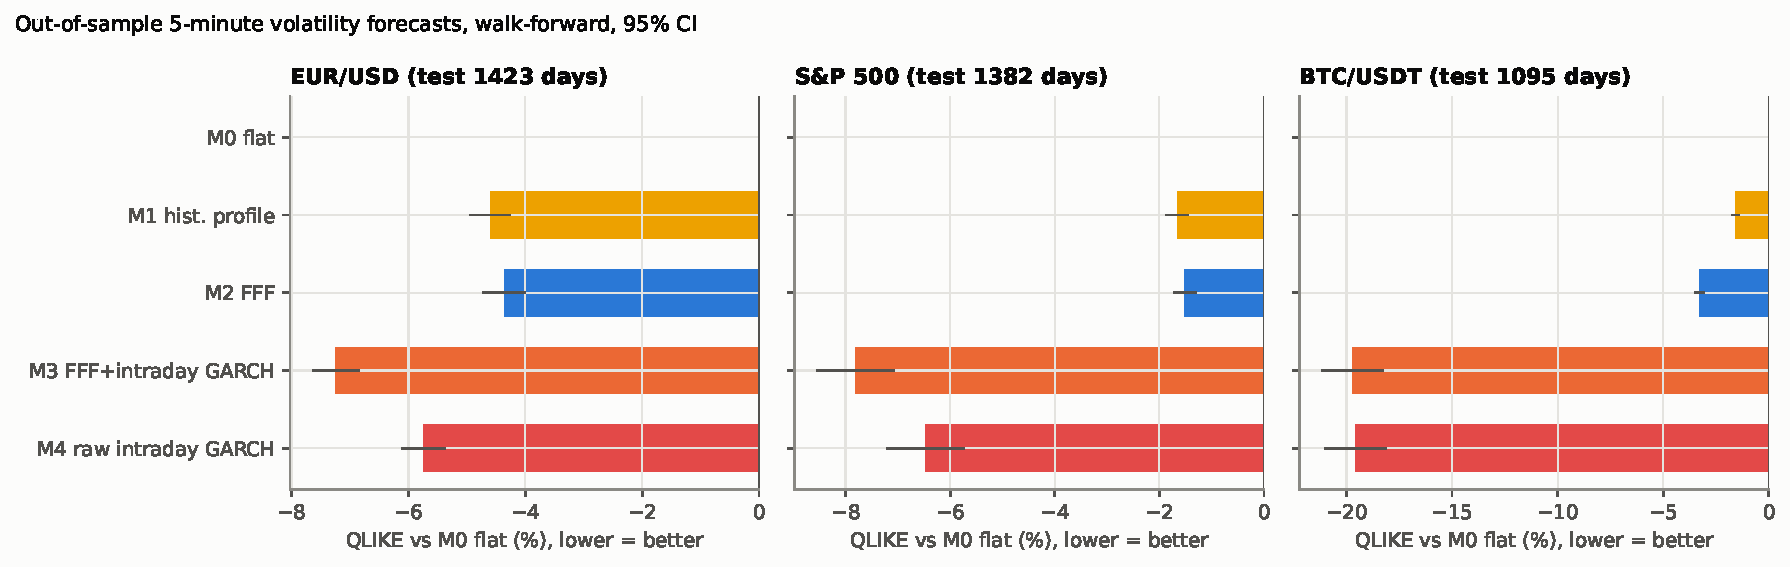
\includegraphics[width=\linewidth]{oos_forecast_qlike.pdf}
\caption{Out-of-sample QLIKE improvement over the flat forecast, with 95\% CIs.}
\label{fig:oos}
\end{figure}

\textbf{Mean-return seasonality (H5).} Table~\ref{tab:trade} and Figure~\ref{fig:trade} report two strategies designed on training data. \emph{FDR intervals} trades the training intervals that survived false-discovery-rate control in the direction of their training mean. For EUR/USD its gross Sharpe ratio is 6.8 in sample (by construction) but 0.4 in both validation and test ($t=0.9$): the in-sample ``discoveries'' are largely noise or have decayed, a textbook illustration of data snooping even after FDR control. \emph{Same-interval momentum} \citep{Heston2010} goes long or short each interval according to the sign of that interval's mean return over the previous 20 days. For EUR/USD it is statistically significant out of sample (test gross Sharpe 4.0, $t=9.0$) and its profits are spread across the day rather than concentrated at the 17:00 rollover. But its break-even cost is 0.05 basis points per round trip, against a realistic cost of 0.6~bp, and the S\&P~500 version breaks even at 0.14~bp against 0.75~bp. The bid-only quotes may also contain spread dynamics that a mid-price would not. Statistically real, economically irrelevant: H5 is supported.

\begin{table}[t]\centering
\caption{Mean-return strategies, base cost. Sharpe ratios annualised. Break-even and assumed cost per round trip in basis points.}
\label{tab:trade}
\tabin{oos_trading}
\end{table}

\begin{figure}[t]\centering
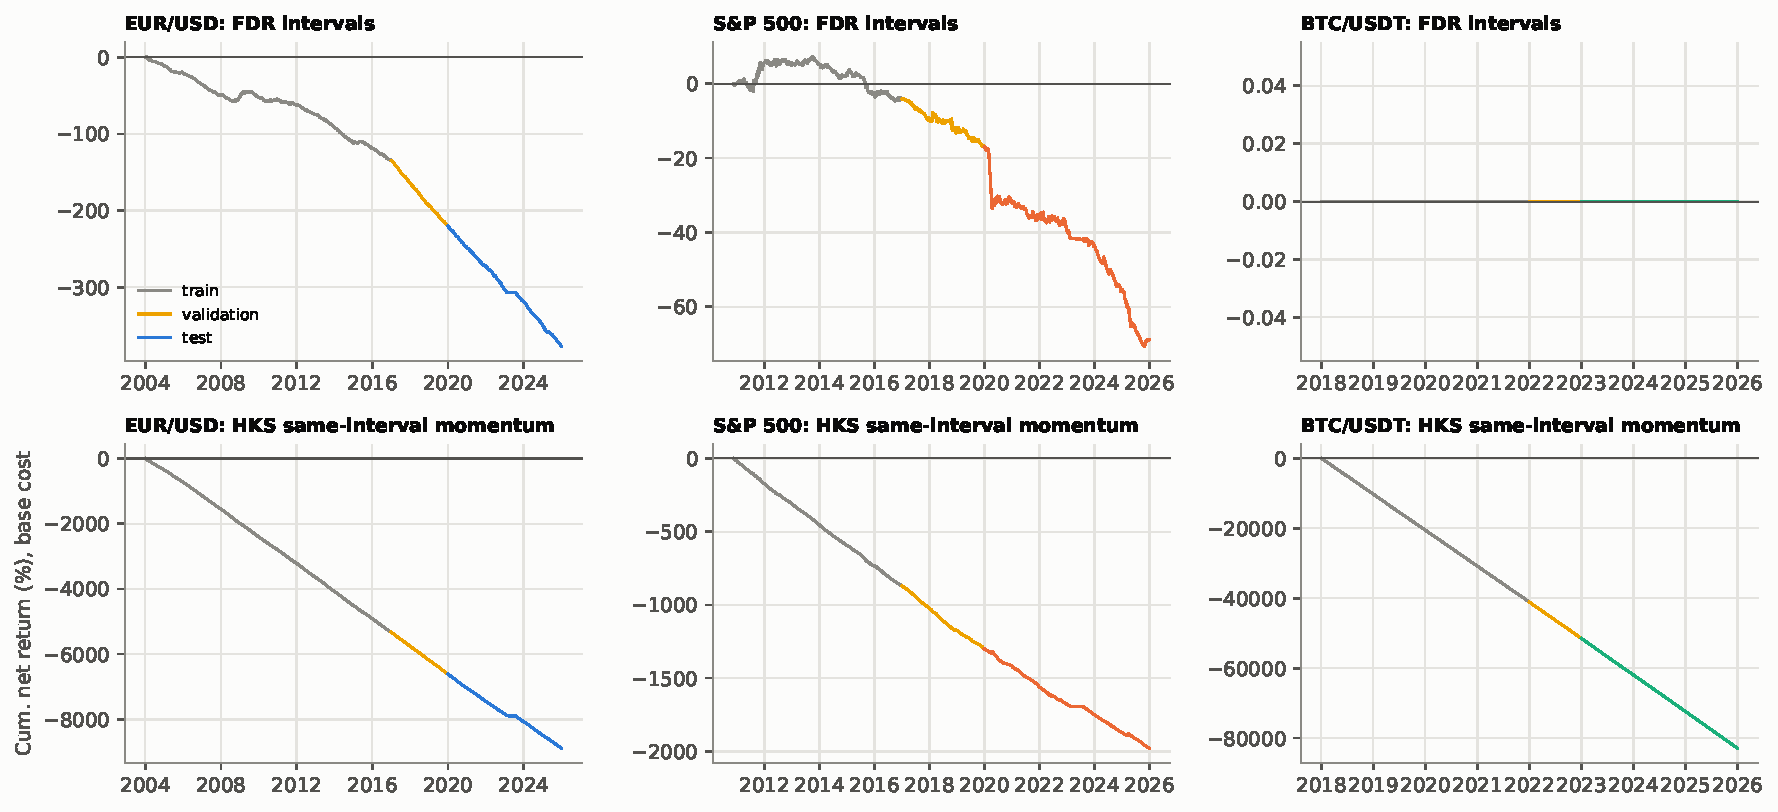
\includegraphics[width=\linewidth]{oos_trading_is_vs_oos.pdf}
\caption{Cumulative \emph{gross} returns of the mean-return strategies: training (grey), validation (yellow), test (asset colour). Net returns are negative throughout for all strategies at realistic costs.}
\label{fig:trade}
\end{figure}

\section{Economic interpretation}
\label{sec:econ}
The economic value of intraday periodicity lies in \emph{second} moments, not first moments. A trader who sizes positions to target a constant risk per 5-minute interval using a forecast that ignores the time of day mis-sizes EUR/USD risk by 33\% on average across intervals, and by more than 25\% in 56\% of intervals. With a historical or FFF profile the error falls to 8--10\% and to 3--7\% of intervals (Figure~\ref{fig:risk}). The same holds for stop-loss placement, execution scheduling and intraday margining: these decisions are all scaled by expected volatility, and the expected volatility of a 5-minute interval can differ by a factor of four or more across the day. For volatility forecasting itself, the out-of-sample gain from combining periodicity filtering with intraday dynamics (M3 vs.\ M0) is 7--8\% of QLIKE for FX and equities and about 20\% for BTC.

The mean-return results tell the opposite story. The periodic structure in volatility does not translate into predictable direction: interval means are tiny relative to their standard deviations, the few that survive multiple-testing control do not survive out of sample, and the one robust effect is an order of magnitude too small to pay the spread. This is what an efficient market with predictable \emph{activity} should look like: participants know when volatility will arrive, and prices adjust so that the timing of volatility carries no free lunch.

The persistence results matter for model builders. In FX, a GARCH model estimated on raw hourly returns would report a volatility half-life of a few hours, while the same data, filtered, give persistence consistent with daily estimates. A risk model calibrated on raw intraday data would badly understate how long volatility shocks last.

\begin{figure}[t]\centering
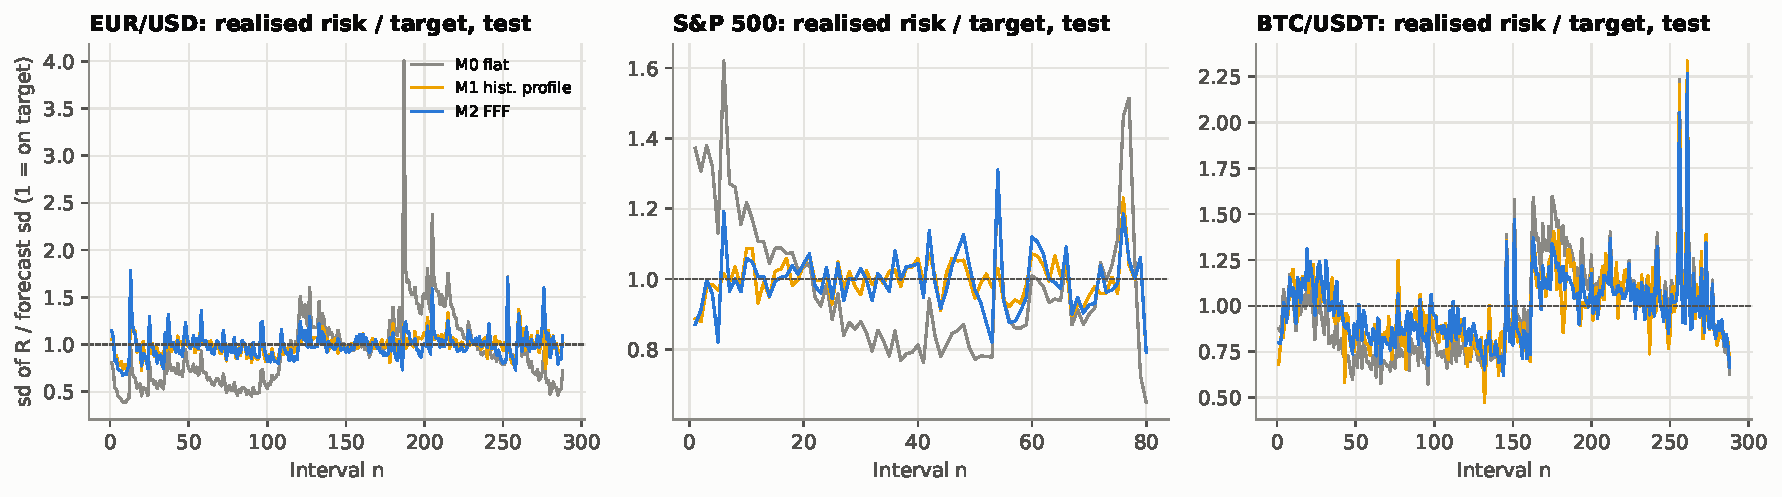
\includegraphics[width=\linewidth]{oos_risk_targeting.pdf}
\caption{Risk targeting, test period: realised standard deviation of $R/\sqrt{v}$ by interval relative to its average (1 = risk on target at every time of day).}
\label{fig:risk}
\end{figure}

\section{Limitations}
\label{sec:lim}
\begin{itemize}
\item \textbf{Data.} The original data are not public, so the replication is methodological, not numerical. EUR/USD and SPXUSD are bid-only HistData series, not midquotes; SPXUSD is a CFD that tracks futures, not the CME contract. HistData has a gap in March--July 2023; affected days are dropped. Dukascopy's rate limits prevented using it beyond validation.
\item \textbf{Volume.} No free consolidated intraday volume exists for FX or the index, so H3 is tested only for BTC (one exchange, Binance).
\item \textbf{Survivorship.} The BTC sample conditions on the survival of Bitcoin and of Binance.
\item \textbf{Model.} Eq.~\eqref{eq:model} assumes a deterministic periodic component; announcement days, half-days and regime changes are only partly captured by dummies and the $\sigma_t$ interaction. GARCH(1,1) is a benchmark, not the true process, as A\&B themselves stress.
\item \textbf{Multiple testing across analyses.} We correct within each family of interval tests but report many analyses; results with $p$-values near 0.05 should be read as suggestive.
\item \textbf{Costs.} Transaction costs are stylised round-trip assumptions; market impact is ignored, which only strengthens the negative trading conclusion.
\item \textbf{Hypothesis, not proof.} Out-of-sample results cover 2020--2025 (2023--2025 for BTC), one particular period. A good backtest is a hypothesis, not a proven strategy.
\end{itemize}

\section{Conclusion}
\label{sec:concl}
Three decades on, A\&B's diagnosis holds. Intraday volatility periodicity is pervasive, stable and economically large, and ignoring it makes GARCH estimates of volatility persistence depend absurdly on the sampling frequency, dramatically so in FX. Filtering the periodic component restores coherence, and the prescription delivers significantly better out-of-sample volatility forecasts and risk targeting for FX, equities and crypto alike. Two refinements emerge for modern data: with discrete prices, the periodic component should be estimated by a zero-robust method such as PPML; and with long samples a non-parametric profile can beat a low-order Fourier form. Intraday seasonality in mean returns, in contrast, is not economically exploitable after costs.

\section{Future research}
\label{sec:future}
\begin{itemize}
\item Model announcement effects explicitly \citep{AB1998} with an economic calendar, and separate jumps from diffusive volatility before estimating the periodic component \citep{Boudt2011}.
\item Combine the periodic filter with heterogeneous-horizon dynamics (HAR, multiplicative component GARCH; \citealp{Corsi2009,Engle2012}) and test whether filtered long memory is genuine or reflects structural breaks.
\item Use midquotes and true volume (paid futures and FX ECN data) to test H3 for FX and equities, and to rule out bid-quote artefacts in same-interval momentum.
\item Extend to single stocks and other crypto assets to study how periodicity varies with liquidity and investor base, and study more formally the 2022--23 migration of BTC volatility to US hours.
\end{itemize}

\clearpage
\section*{Reproducibility}
Code, figures, tables and this paper are in the accompanying repository. \texttt{make all} (or \texttt{./reproduce.sh}) downloads the data from the original free sources, validates it, and regenerates every number, table and figure; Python~3.12 dependencies are pinned in \texttt{uv.lock}. Random seeds are fixed.

\bibliographystyle{plainnat}
\begin{thebibliography}{99}
\bibitem[Admati and Pfleiderer(1988)]{AdmatiPfleiderer1988} Admati, A.R., Pfleiderer, P. (1988). A theory of intraday patterns: volume and price variability. \emph{Review of Financial Studies} 1(1), 3--40.
\bibitem[Andersen and Bollerslev(1997)]{AB1997} Andersen, T.G., Bollerslev, T. (1997). Intraday periodicity and volatility persistence in financial markets. \emph{Journal of Empirical Finance} 4(2--3), 115--158.
\bibitem[Andersen and Bollerslev(1998)]{AB1998} Andersen, T.G., Bollerslev, T. (1998). Deutsche mark--dollar volatility: intraday activity patterns, macroeconomic announcements, and longer run dependencies. \emph{Journal of Finance} 53(1), 219--265.
\bibitem[Andersen et~al.(2003)]{Andersen2003} Andersen, T.G., Bollerslev, T., Diebold, F.X., Vega, C. (2003). Micro effects of macro announcements: real-time price discovery in foreign exchange. \emph{American Economic Review} 93(1), 38--62.
\bibitem[Benjamini and Hochberg(1995)]{BenjaminiHochberg1995} Benjamini, Y., Hochberg, Y. (1995). Controlling the false discovery rate: a practical and powerful approach to multiple testing. \emph{Journal of the Royal Statistical Society B} 57(1), 289--300.
\bibitem[Bollerslev(1986)]{Bollerslev1986} Bollerslev, T. (1986). Generalized autoregressive conditional heteroskedasticity. \emph{Journal of Econometrics} 31(3), 307--327.
\bibitem[Bollerslev and Wooldridge(1992)]{BollerslevWooldridge1992} Bollerslev, T., Wooldridge, J.M. (1992). Quasi-maximum likelihood estimation and inference in dynamic models with time-varying covariances. \emph{Econometric Reviews} 11(2), 143--172.
\bibitem[Boudt et~al.(2011)]{Boudt2011} Boudt, K., Croux, C., Laurent, S. (2011). Robust estimation of intraweek periodicity in volatility and jump detection. \emph{Journal of Empirical Finance} 18(2), 353--367.
\bibitem[Corsi(2009)]{Corsi2009} Corsi, F. (2009). A simple approximate long-memory model of realized volatility. \emph{Journal of Financial Econometrics} 7(2), 174--196.
\bibitem[Dacorogna et~al.(1993)]{Dacorogna1993} Dacorogna, M.M., M\"uller, U.A., Nagler, R.J., Olsen, R.B., Pictet, O.V. (1993). A geographical model for the daily and weekly seasonal volatility in the foreign exchange market. \emph{Journal of International Money and Finance} 12(4), 413--438.
\bibitem[Diebold and Mariano(1995)]{DieboldMariano1995} Diebold, F.X., Mariano, R.S. (1995). Comparing predictive accuracy. \emph{Journal of Business \& Economic Statistics} 13(3), 253--263.
\bibitem[Drost and Nijman(1993)]{DrostNijman1993} Drost, F.C., Nijman, T.E. (1993). Temporal aggregation of GARCH processes. \emph{Econometrica} 61(4), 909--927.
\bibitem[Engle and Sokalska(2012)]{Engle2012} Engle, R.F., Sokalska, M.E. (2012). Forecasting intraday volatility in the US equity market. Multiplicative component GARCH. \emph{Journal of Financial Econometrics} 10(1), 54--83.
\bibitem[Gallant(1981)]{Gallant1981} Gallant, A.R. (1981). On the bias in flexible functional forms and an essentially unbiased form: the Fourier flexible form. \emph{Journal of Econometrics} 15(2), 211--245.
\bibitem[Gao et~al.(2018)]{Gao2018} Gao, L., Han, Y., Li, S.Z., Zhou, G. (2018). Market intraday momentum. \emph{Journal of Financial Economics} 129(2), 394--414.
\bibitem[Harris(1986)]{Harris1986} Harris, L. (1986). A transaction data study of weekly and intradaily patterns in stock returns. \emph{Journal of Financial Economics} 16(1), 99--117.
\bibitem[Harvey et~al.(2016)]{HarveyLiuZhu2016} Harvey, C.R., Liu, Y., Zhu, H. (2016). \ldots and the cross-section of expected returns. \emph{Review of Financial Studies} 29(1), 5--68.
\bibitem[Heston et~al.(2010)]{Heston2010} Heston, S.L., Korajczyk, R.A., Sadka, R. (2010). Intraday patterns in the cross-section of stock returns. \emph{Journal of Finance} 65(4), 1369--1407.
\bibitem[K\"unsch(1989)]{Kunsch1989} K\"unsch, H.R. (1989). The jackknife and the bootstrap for general stationary observations. \emph{Annals of Statistics} 17(3), 1217--1241.
\bibitem[M\"uller et~al.(1997)]{Muller1997} M\"uller, U.A., Dacorogna, M.M., Dav\'e, R.D., Olsen, R.B., Pictet, O.V., von Weizs\"acker, J.E. (1997). Volatilities of different time resolutions --- analyzing the dynamics of market components. \emph{Journal of Empirical Finance} 4(2--3), 213--239.
\bibitem[Newey and West(1987)]{NeweyWest1987} Newey, W.K., West, K.D. (1987). A simple, positive semi-definite, heteroskedasticity and autocorrelation consistent covariance matrix. \emph{Econometrica} 55(3), 703--708.
\bibitem[Patton(2011)]{Patton2011} Patton, A.J. (2011). Volatility forecast comparison using imperfect volatility proxies. \emph{Journal of Econometrics} 160(1), 246--256.
\bibitem[Santos Silva and Tenreyro(2006)]{SantosSilva2006} Santos Silva, J.M.C., Tenreyro, S. (2006). The log of gravity. \emph{Review of Economics and Statistics} 88(4), 641--658.
\bibitem[Taylor and Xu(1997)]{TaylorXu1997} Taylor, S.J., Xu, X. (1997). The incremental volatility information in one million foreign exchange quotations. \emph{Journal of Empirical Finance} 4(4), 317--340.
\bibitem[Wood et~al.(1985)]{Wood1985} Wood, R.A., McInish, T.H., Ord, J.K. (1985). An investigation of transactions data for NYSE stocks. \emph{Journal of Finance} 40(3), 723--739.
\end{thebibliography}

\clearpage
\appendix
\section{Additional figures}
\begin{figure}[h]\centering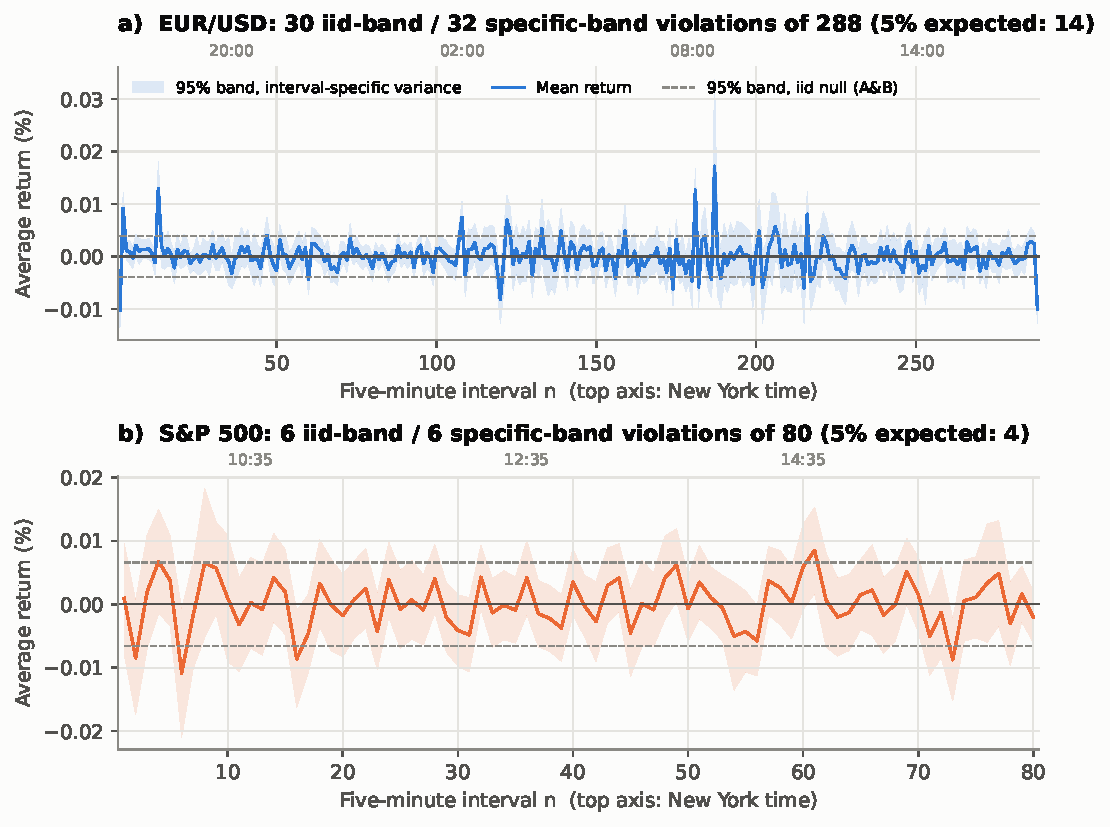
\includegraphics[width=0.85\linewidth]{rep_fig1_mean_returns.pdf}
\caption{Average returns by interval with A\&B's constant iid band (dashed) and interval-specific 95\% bands (A\&B Fig.~1).}\label{fig:rep1}\end{figure}
\begin{figure}[h]\centering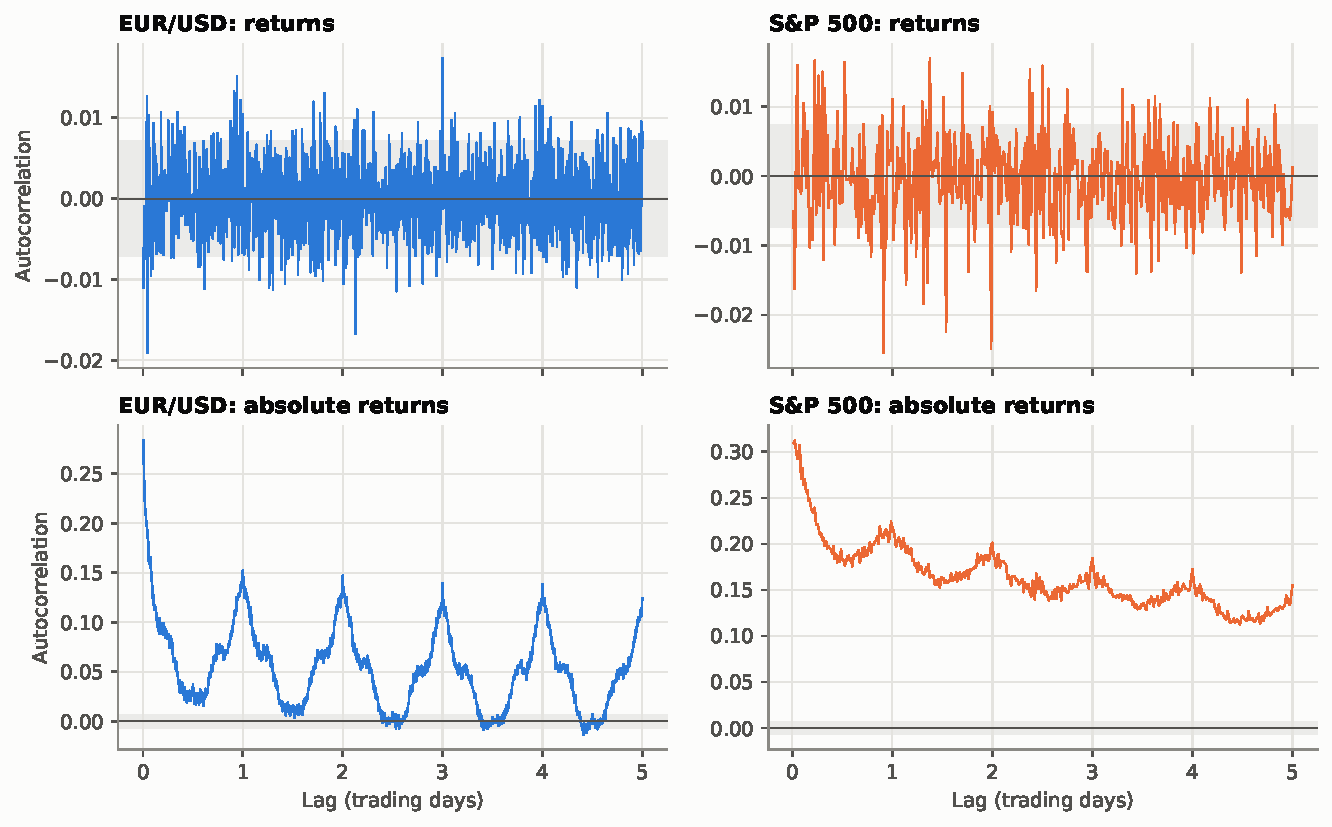
\includegraphics[width=0.95\linewidth]{rep_fig3_4_correlograms.pdf}
\caption{Five-day correlograms of returns and absolute returns (A\&B Figs.~3--4).}\end{figure}
\begin{figure}[h]\centering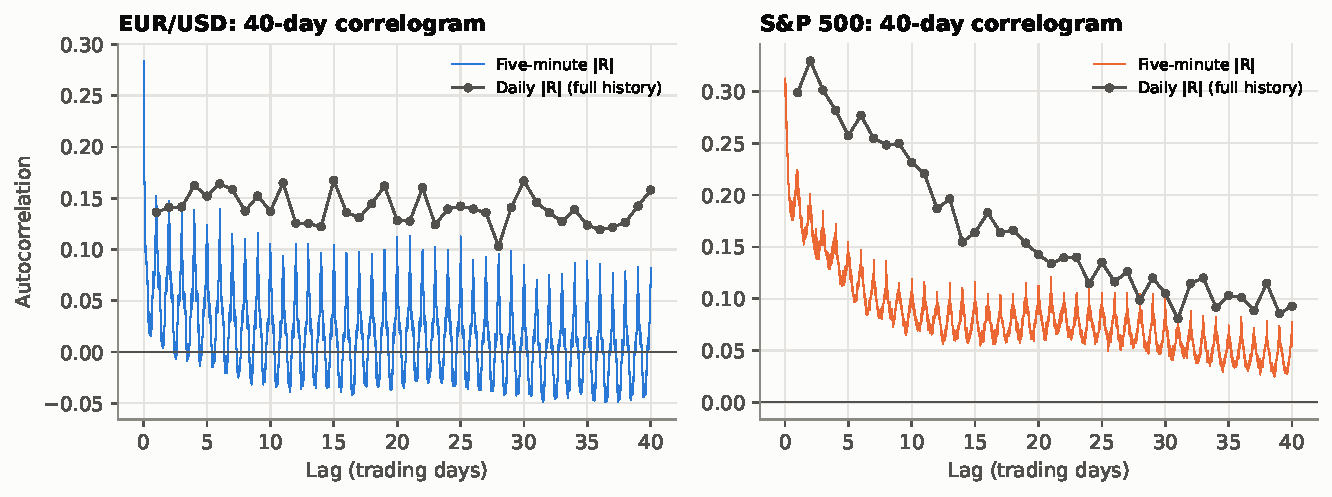
\includegraphics[width=0.95\linewidth]{rep_fig5_daily_vs_intraday.pdf}
\caption{40-day correlogram of 5-minute $|R|$ vs.\ daily $|R|$ (A\&B Fig.~5).}\end{figure}
\begin{figure}[h]\centering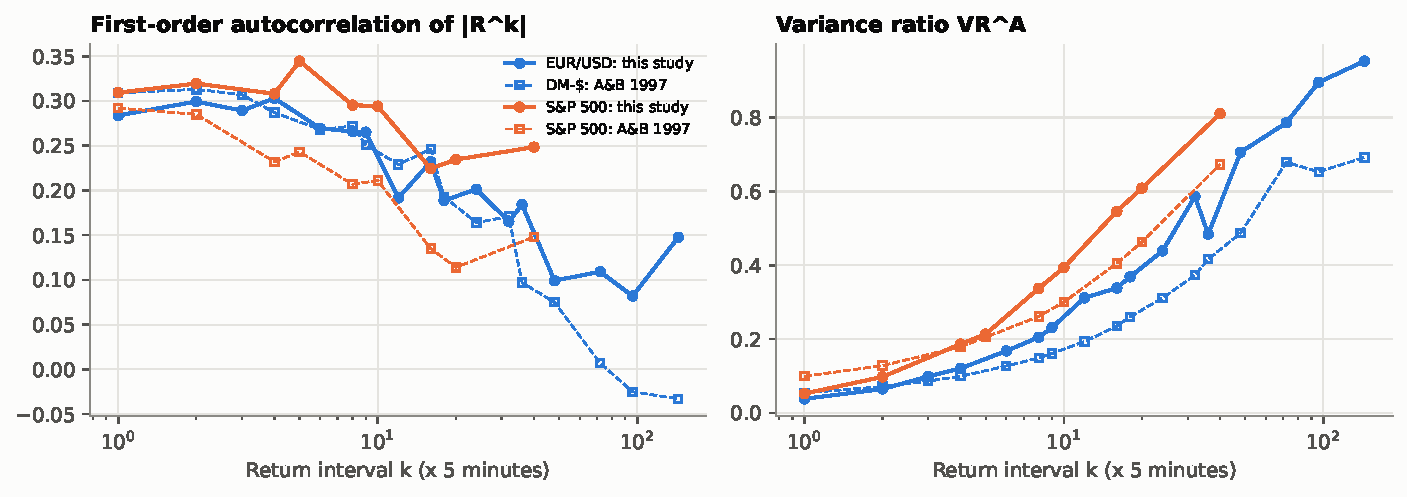
\includegraphics[width=0.95\linewidth]{rep_table1_comparison.pdf}
\caption{A\&B Table~1 comparison: $\rho_1^A$ and $VR^A$ by frequency.}\end{figure}
\begin{figure}[h]\centering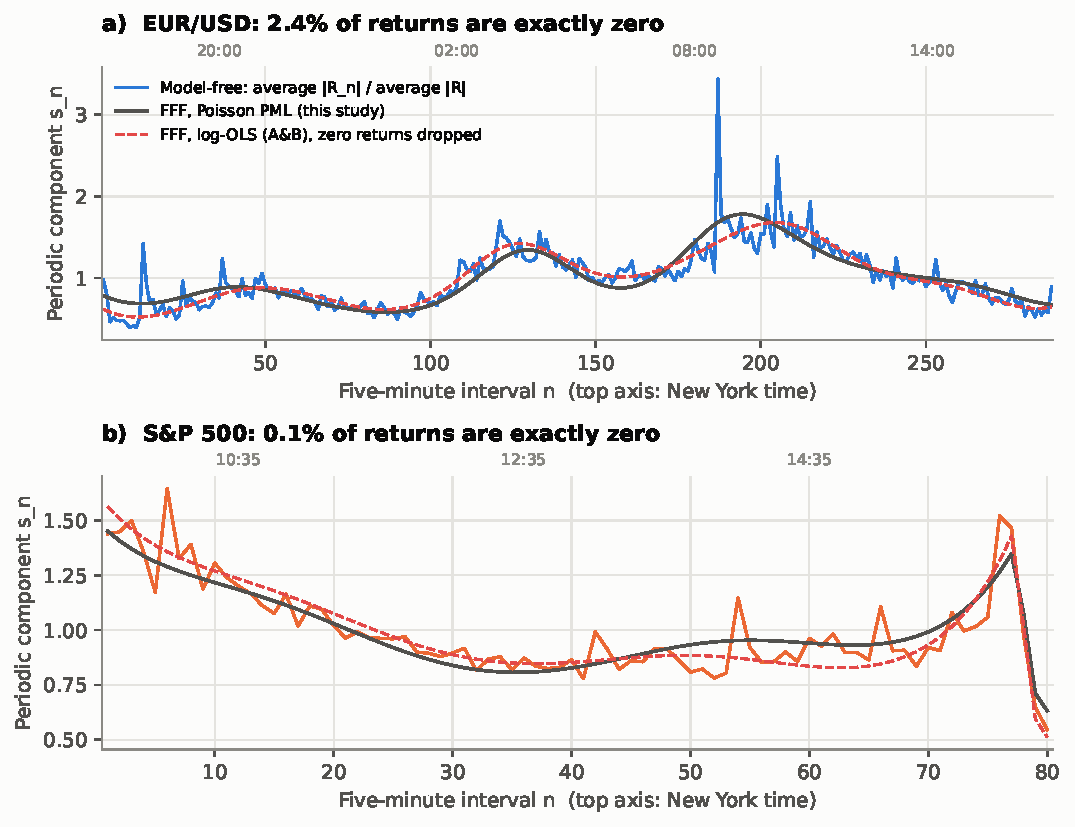
\includegraphics[width=0.85\linewidth]{rep_fig_estimator_comparison.pdf}
\caption{Periodic component: model-free profile vs.\ FFF by PPML and by A\&B's log-OLS.}\label{fig:est}\end{figure}
\begin{figure}[h]\centering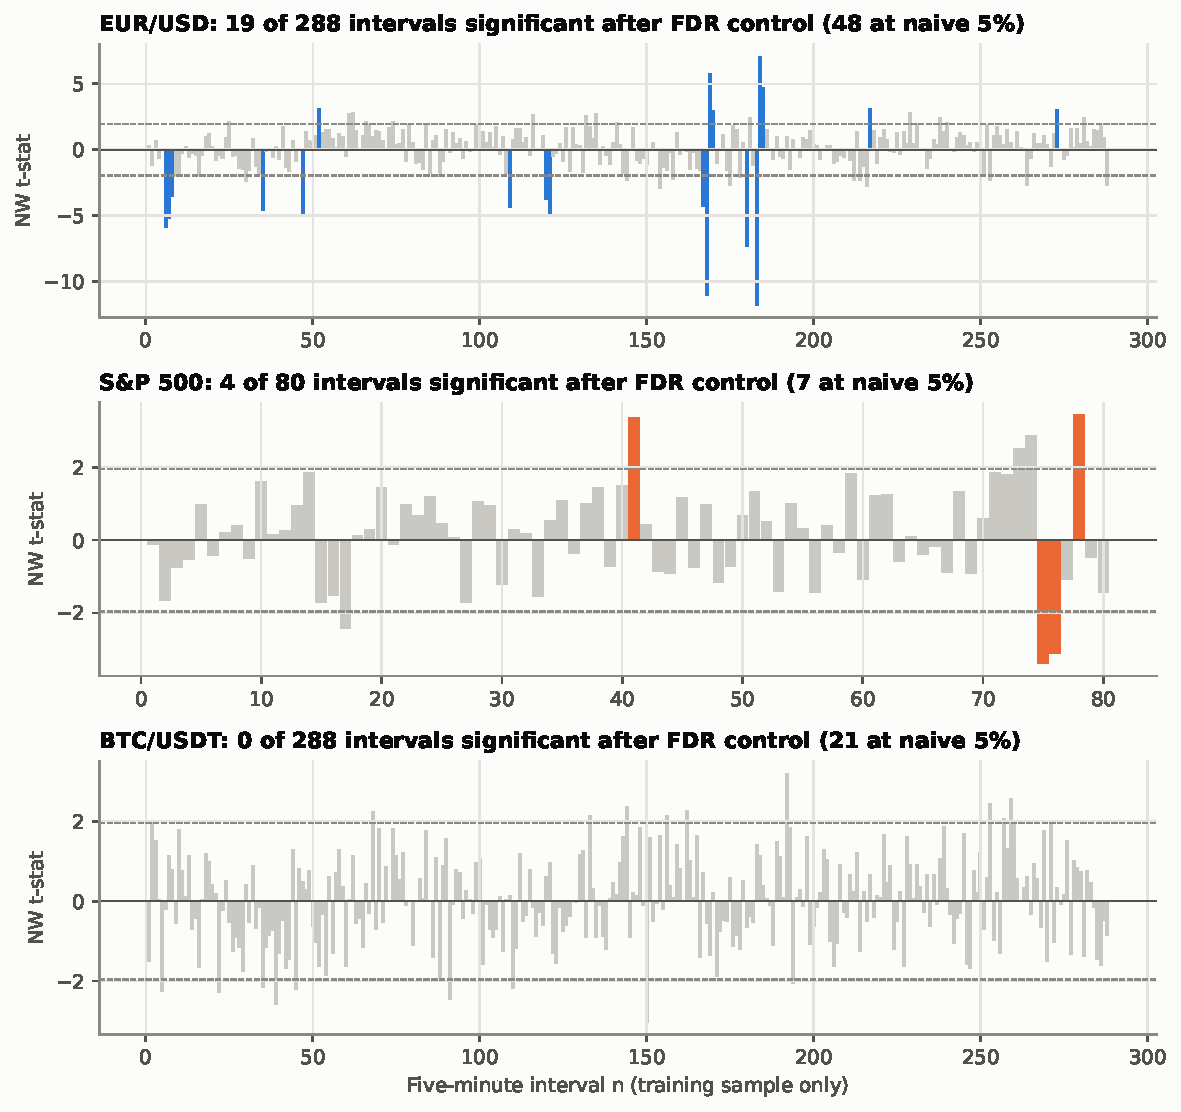
\includegraphics[width=0.85\linewidth]{ext_e3_mean_return_tstats.pdf}
\caption{Per-interval mean-return Newey--West $t$-statistics, training data; coloured bars survive BH-FDR control.}\end{figure}
\begin{figure}[h]\centering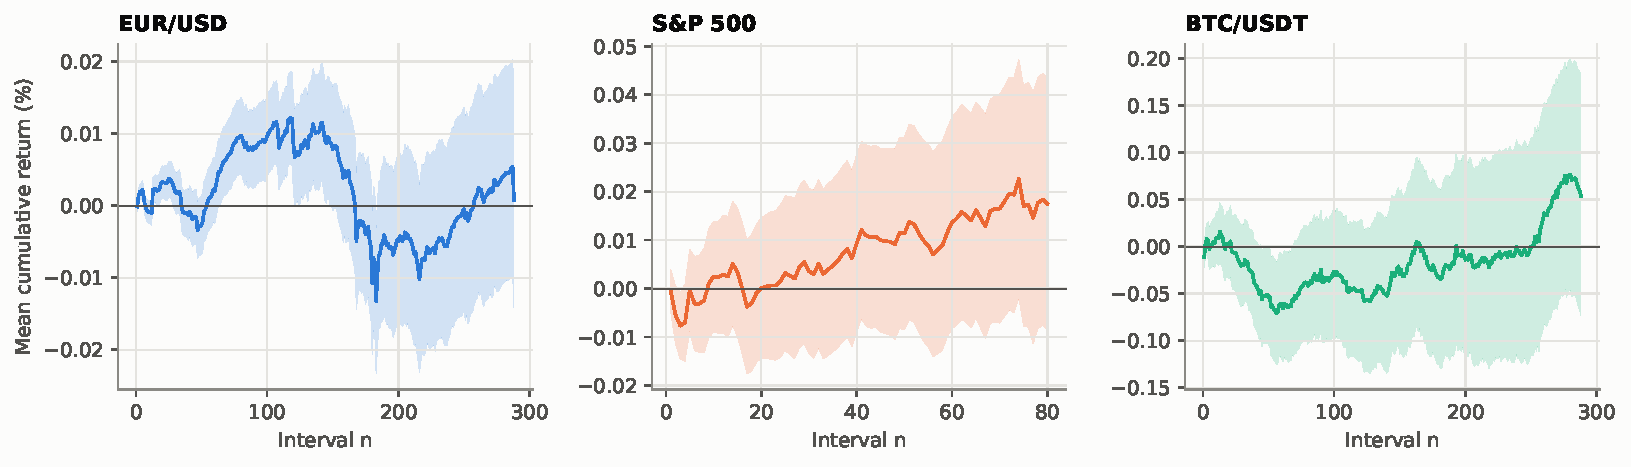
\includegraphics[width=0.95\linewidth]{ext_e3_cumulative_return_path.pdf}
\caption{Average cumulative intraday return path with 95\% CI, full samples.}\end{figure}
\begin{figure}[h]\centering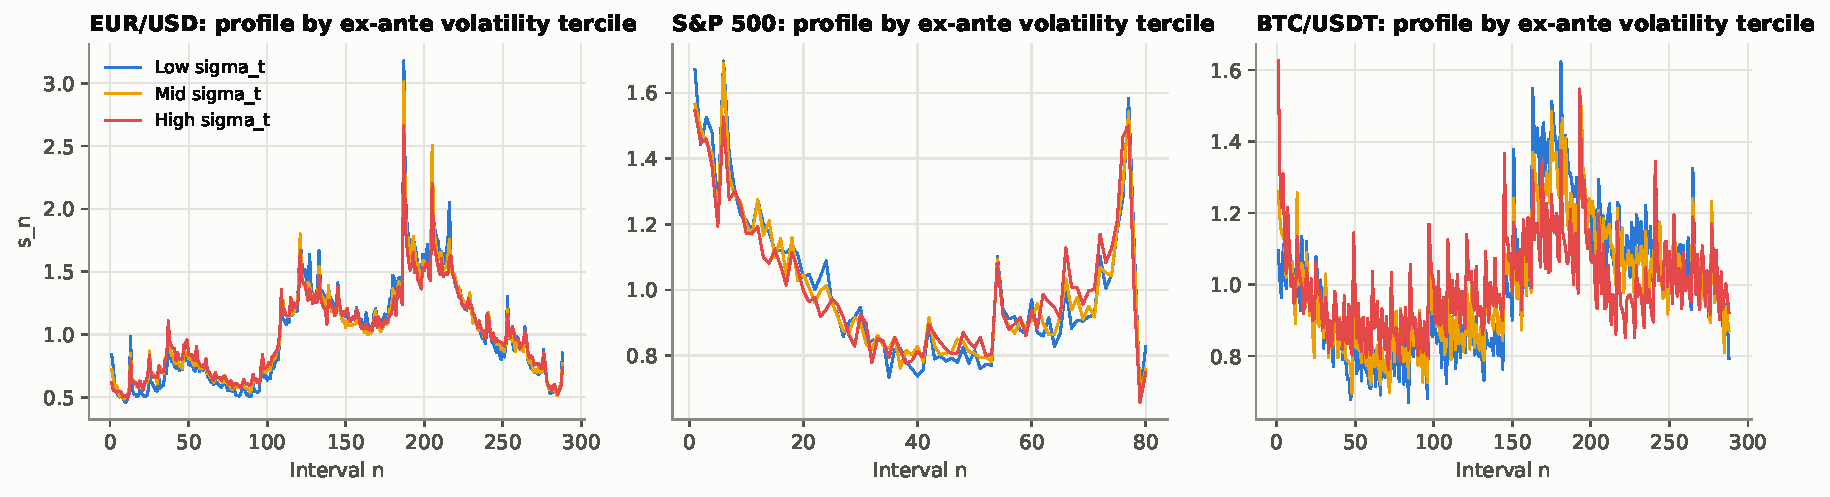
\includegraphics[width=0.95\linewidth]{ext_e5a_profile_by_vol_regime.pdf}
\caption{Volatility profile by tercile of ex-ante daily volatility.}\end{figure}
\begin{figure}[h]\centering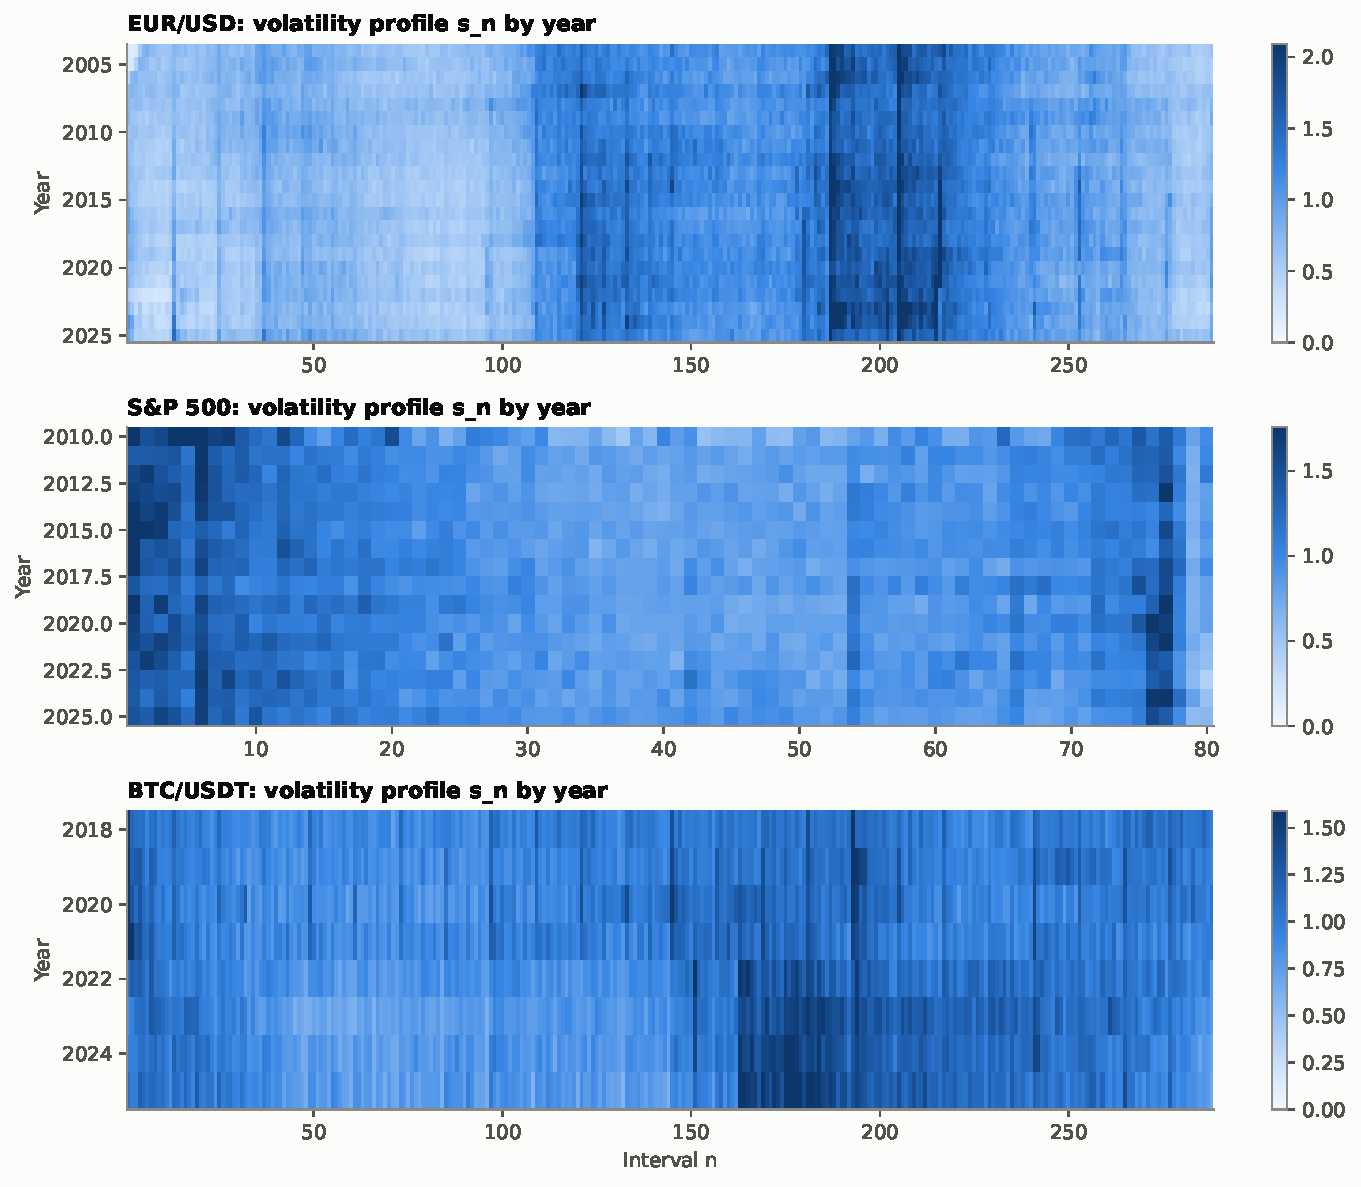
\includegraphics[width=0.8\linewidth]{ext_e5b_profile_stability_by_year.pdf}
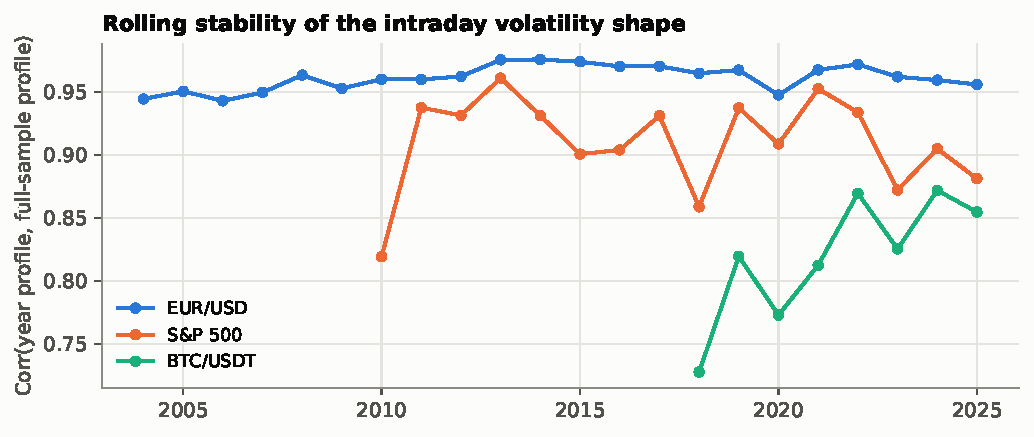
\includegraphics[width=0.6\linewidth]{ext_e5c_profile_stability_corr.pdf}
\caption{Stability of the intraday volatility shape by calendar year.}\label{fig:stab}\end{figure}
\begin{figure}[h]\centering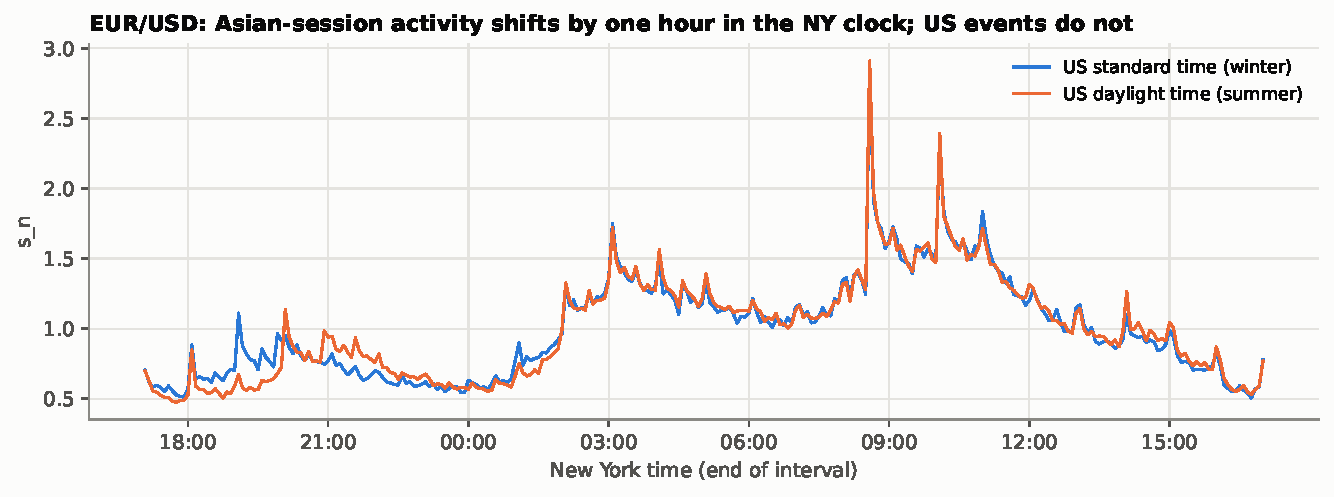
\includegraphics[width=0.85\linewidth]{ext_e5d_eurusd_dst.pdf}
\caption{EUR/USD in the New York clock, US winter vs.\ summer: Asian-session activity shifts by one hour, New York events do not.}\end{figure}
\begin{figure}[h]\centering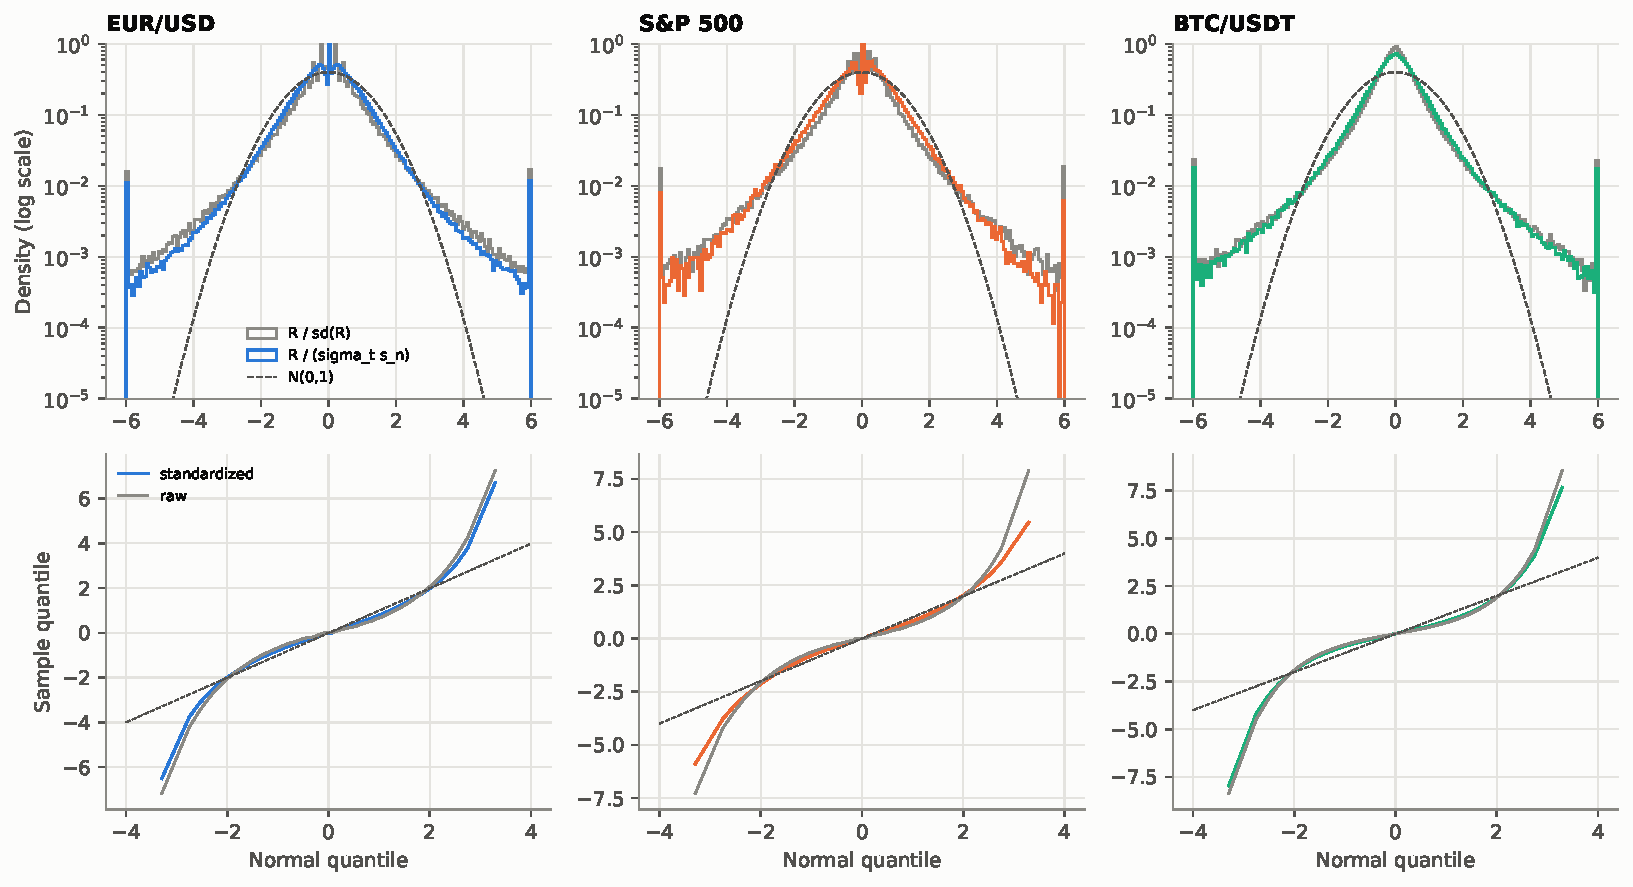
\includegraphics[width=0.95\linewidth]{ext_e6_distributions.pdf}
\caption{Distribution of raw and standardised 5-minute returns (log density and QQ plots).}\label{fig:dist}\end{figure}
\begin{figure}[h]\centering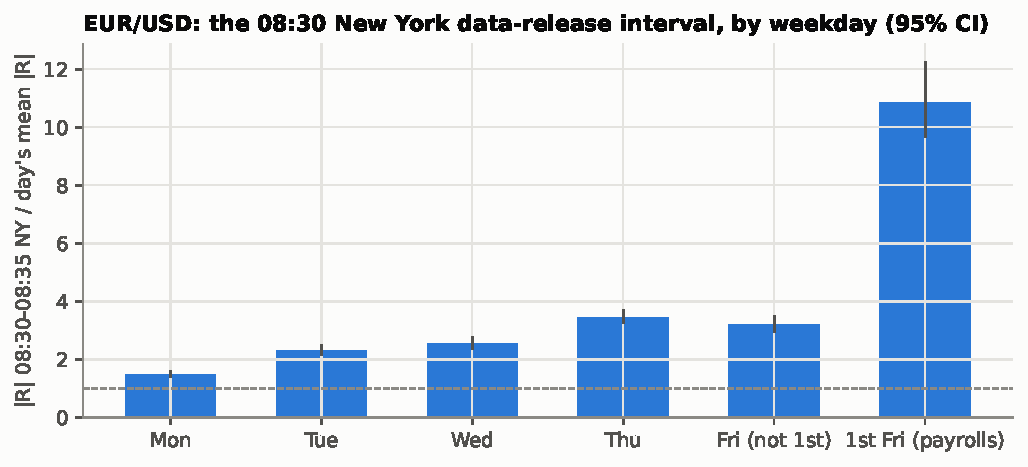
\includegraphics[width=0.7\linewidth]{ext_e7_0830_effect.pdf}
\caption{EUR/USD 08:30--08:35 New York interval volatility relative to the day's mean, by weekday and on payroll Fridays (95\% CI).}\label{fig:0830}\end{figure}
\begin{figure}[h]\centering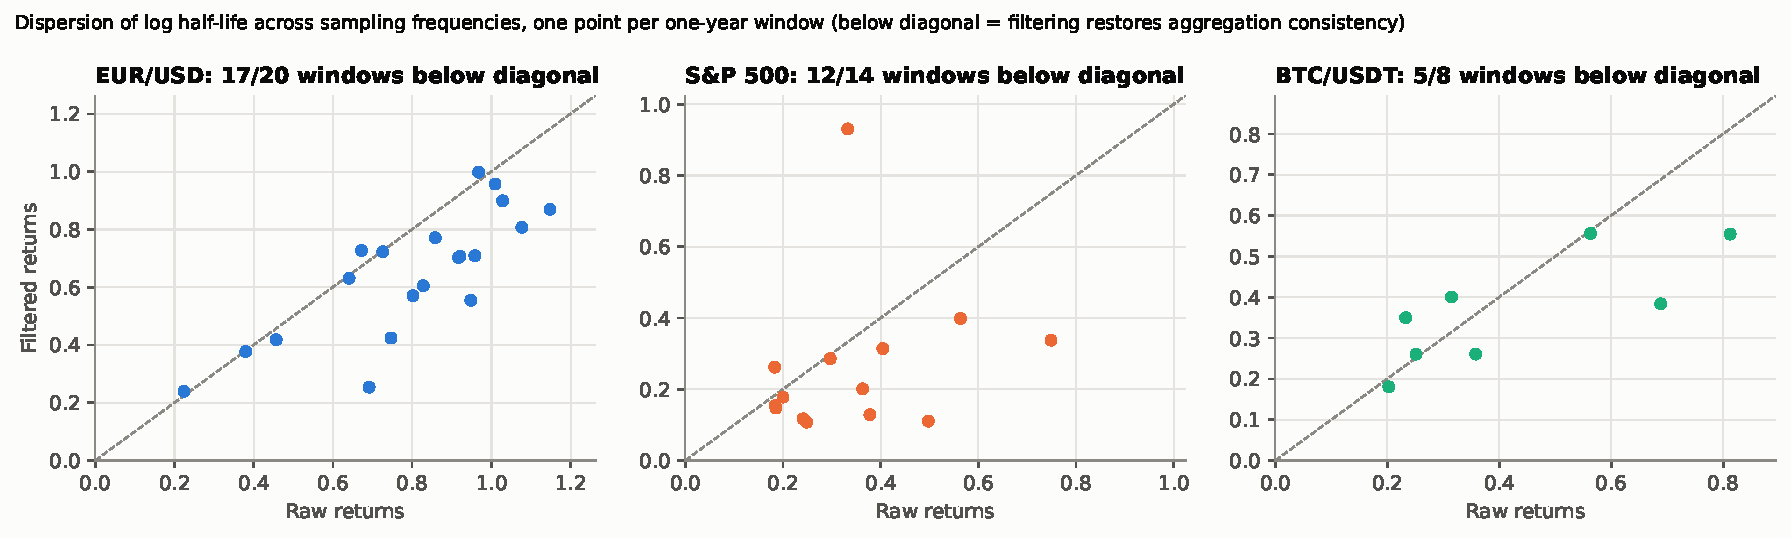
\includegraphics[width=0.95\linewidth]{rob_r1_dispersion_scatter.pdf}
\caption{Aggregation consistency, raw vs.\ filtered, one point per one-year window.}\end{figure}
\begin{figure}[h]\centering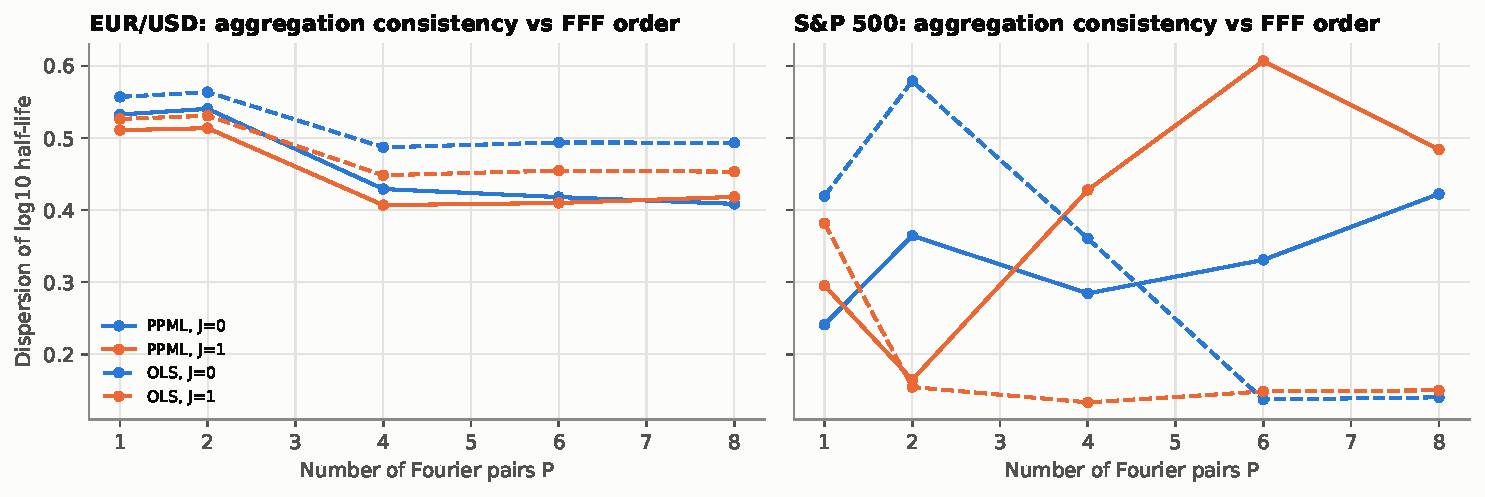
\includegraphics[width=0.85\linewidth]{rob_r2_fff_spec.pdf}
\caption{Sensitivity of aggregation consistency to the FFF order and estimator.}\label{fig:spec}\end{figure}
\end{document}
